%%%%%%%%%%%%%%%%%%%%%%%%%%%%%%%%%%%%%%%%%%%%%%%%%%%%%%%%%%%%%%%%%%%%%%%%%%%%
% AGUJournalTemplate.tex: this template file is for articles formatted with LaTeX
%
% This file includes commands and instructions
% given in the order necessary to produce a final output that will
% satisfy AGU requirements, including customized APA reference formatting.
%
% You may copy this file and give it your
% article name, and enter your text.
%
% guidelines and troubleshooting are here: 

%% To submit your paper:
\documentclass[draft]{agujournal2019}
\usepackage{url} %this package should fix any errors with URLs in refs.
\usepackage{graphicx}
\usepackage{lineno}
\usepackage[inline]{trackchanges} %for better track changes. finalnew option will compile document with changes incorporated.
\usepackage{soul}
\linenumbers
%%%%%%%
% As of 2018 we recommend use of the TrackChanges package to mark revisions.
% The trackchanges package adds five new LaTeX commands:
%
%  \note[editor]{The note}
%  \annote[editor]{Text to annotate}{The note}
%  \add[editor]{Text to add}
%  \remove[editor]{Text to remove}
%  \change[editor]{Text to remove}{Text to add}
%
% complete documentation is here: http://trackchanges.sourceforge.net/
%%%%%%%

\draftfalse

%% Enter journal name below.
%% Choose from this list of Journals:
%
% JGR: Atmospheres
% JGR: Biogeosciences
% JGR: Earth Surface
% JGR: Oceans
% JGR: Planets
% JGR: Solid Earth
% JGR: Space Physics
% Global Biogeochemical Cycles
% Geophysical Research Letters
% Paleoceanography and Paleoclimatology
% Radio Science
% Reviews of Geophysics
% Tectonics
% Space Weather
% Water Resources Research
% Geochemistry, Geophysics, Geosystems
% Journal of Advances in Modeling Earth Systems (JAMES)
% Earth's Future
% Earth and Space Science
% Geohealth
%
% ie, \journalname{Water Resources Research}

\journalname{JGR: Solid Earth}


\begin{document}

%%%%%%%%%%%%%%%%%%%%%%%%%%%%%%%%%%%%%%%%%%%%%%%
%  TITLE
%
% (A title should be specific, informative, and brief. Use
% abbreviations only if they are defined in the abstract. Titles that
% start with general keywords then specific terms are optimized in
% searches)
%
%%%%%%%%%%%%%%%%%%%%%%%%%%%%%%%%%%%%%%%%%%%%%%%

% Example: \title{This is a test title}

\title{Reactive Transport Control on Finite-Offset Seismoelectric Interface Responses During Carbonate Dissolution}

%%%%%%%%%%%%%%%%%%%%%%%%%%%%%%%%%%%%%%%%%%%%%%%
%
%  AUTHORS AND AFFILIATIONS
%
%%%%%%%%%%%%%%%%%%%%%%%%%%%%%%%%%%%%%%%%%%%%%%%

% Authors are individuals who have significantly contributed to the
% research and preparation of the article. Group authors are allowed, if
% each author in the group is separately identified in an appendix.)

% List authors by first name or initial followed by last name and
% separated by commas. Use \affil{} to number affiliations, and
% \thanks{} for author notes.
% Additional author notes should be indicated with \thanks{} (for
% example, for current addresses).

% Example: \authors{A. B. Author\affil{1}\thanks{Current address, Antartica}, B. C. Author\affil{2,3}, and D. E.
% Author\affil{3,4}\thanks{Also funded by Monsanto.}}

\authors{Author Name\affil{1}}


% \affiliation{1}{First Affiliation}
% \affiliation{2}{Second Affiliation}
% \affiliation{3}{Third Affiliation}
% \affiliation{4}{Fourth Affiliation}

\affiliation{1}{Affiliation Address}
%(repeat as many times as is necessary)


% Corresponding author mailing address and e-mail address:

% (include name and email addresses of the corresponding author.  More
% than one corresponding author is allowed in this LaTeX file and for
% publication; but only one corresponding author is allowed in our
% editorial system.)

% Example: \correspondingauthor{First and Last Name}{email@address.edu}

\correspondingauthor{Corresponding Author}{email@address.edu}



%%%%%%%%%%%%%%%%%%%%%%%%%%%%%%%%%%%%%%%%%%%%%%%
% KEY POINTS
%%%%%%%%%%%%%%%%%%%%%%%%%%%%%%%%%%%%%%%%%%%%%%%
%  List up to three key points (at least one is required)
%  Key Points summarize the main points and conclusions of the article
%  Each must be 140 characters or fewer with no special characters or punctuation and must be complete sentences

% Example:
% \begin{keypoints}
% \item	List up to three key points (at least one is required)
% \item	Key Points summarize the main points and conclusions of the article
% \item	Each must be 140 characters or fewer with no special characters or punctuation and must be complete sentences
% \end{keypoints}

\begin{keypoints}
\item Carbonate dissolution changes hydraulic connectivity and pore fluid conductivity through different pathways
\item Conductivity growth can suppress electrokinetic coupling even when permeability increases
\item Finite offset waveforms preserve the coefficient level weakening of interface electromagnetic responses
\end{keypoints}

%%%%%%%%%%%%%%%%%%%%%%%%%%%%%%%%%%%%%%%%%%%%%%%
%
%  ABSTRACT and PLAIN LANGUAGE SUMMARY
%
% A good Abstract will begin with a short description of the problem
% being addressed, briefly describe the new data or analyses, then
% briefly states the main conclusion(s) and how they are supported and
% uncertainties.

% The Plain Language Summary should be written for a broad audience,
% including journalists and the science-interested public, that will not have 
% a background in your field.
%
% A Plain Language Summary is required in GRL, JGR: Planets, JGR: Biogeosciences,
% JGR: Oceans, G-Cubed, Reviews of Geophysics, and JAMES.
% see http://sharingscience.agu.org/creating-plain-language-summary/)
%
%%%%%%%%%%%%%%%%%%%%%%%%%%%%%%%%%%%%%%%%%%%%%%%

%% \begin{abstract} starts the second page

\begin{abstract}
Seismoelectric interface responses can be sensitive to hydraulic and electrical contrasts, but it remains unclear how reactive transport changes these signals as pore networks dissolve.
Here we map reactive transport outputs for carbonate dissolution into dynamic electrokinetic properties, Schakel-type interface conversion coefficients, and Liu-type finite-offset waveform synthesis.
The simulations indicate that dissolution increases porosity and permeability, but higher Peclet number cases also produce stronger pore-fluid conductivity growth and a marked decrease in the dynamic coupling coefficient.
As a result, the interface conversion coefficients and post-$T_0$ waveform amplitudes decrease most strongly in the cases with the largest permeability increase.
These results suggest that seismoelectric monitoring of dissolution should account for the competition between hydraulic connectivity and electrical leakage, rather than interpreting permeability growth alone.
\end{abstract}

\section*{Plain Language Summary}
When rock dissolves, pores can become more connected and fluids can move more easily.
At the same time, the fluid in the pores can become more electrically conductive.
These two changes have opposite effects on seismoelectric signals, which are electrical signals produced when seismic waves pass through water-filled porous rocks.
This study uses numerical simulations to test how carbonate dissolution changes these signals.
The results show that stronger flow pathways do not necessarily produce stronger seismoelectric responses, because increased fluid conductivity can weaken the electrokinetic source.


%%%%%%%%%%%%%%%%%%%%%%%%%%%%%%%%%%%%%%%%%%%%%%%
%
%  BODY TEXT
%
%%%%%%%%%%%%%%%%%%%%%%%%%%%%%%%%%%%%%%%%%%%%%%%

%%% Suggested section heads:
% \section{Introduction}
%
% The main text should start with an introduction. Except for short
% manuscripts (such as comments and replies), the text should be divided
% into sections, each with its own heading.

% Headings should be sentence fragments and do not begin with a
% lowercase letter or number. Examples of good headings are:

% \section{Materials and Methods}
% Here is text on Materials and Methods.
%
% \subsection{A descriptive heading about methods}
% More about Methods.
%
% \section{Data} (Or section title might be a descriptive heading about data)
%
% \section{Results} (Or section title might be a descriptive heading about the
% results)
%
% \section{Conclusions}


\section{Introduction}

Seismoelectric interface responses provide a way to connect seismic wave propagation with hydraulic and electrical contrasts in porous media.
Previous work has shown that these responses can contain information about permeability, saturation, salinity, and layered structure, but most interpretations treat the material state as fixed.

Reactive transport studies show that mineral dissolution can reorganize pore geometry, flow pathways, and pore-fluid chemistry over a much longer time scale.
For carbonate media, these changes can increase porosity and permeability while also changing tortuosity and electrical conductivity.

The central challenge is that these changes do not affect the seismoelectric source in the same direction.
Permeability growth can strengthen hydraulic communication, whereas conductivity growth can reduce the relative electrokinetic coupling and weaken the interfacial current imbalance.

This study tests how this competition is transferred from reactive transport outputs to dynamic electrokinetic parameters, interface conversion coefficients, and finite-offset waveform amplitudes.
We distinguish dissolution time, which describes chemical evolution, from waveform time, which describes the microsecond-scale response of one evolved material state.
Figure~\ref{fig:workflow} defines the finite-offset source-receiver geometry and summarizes the coupled workflow across these two time scales.

\begin{figure}
\noindent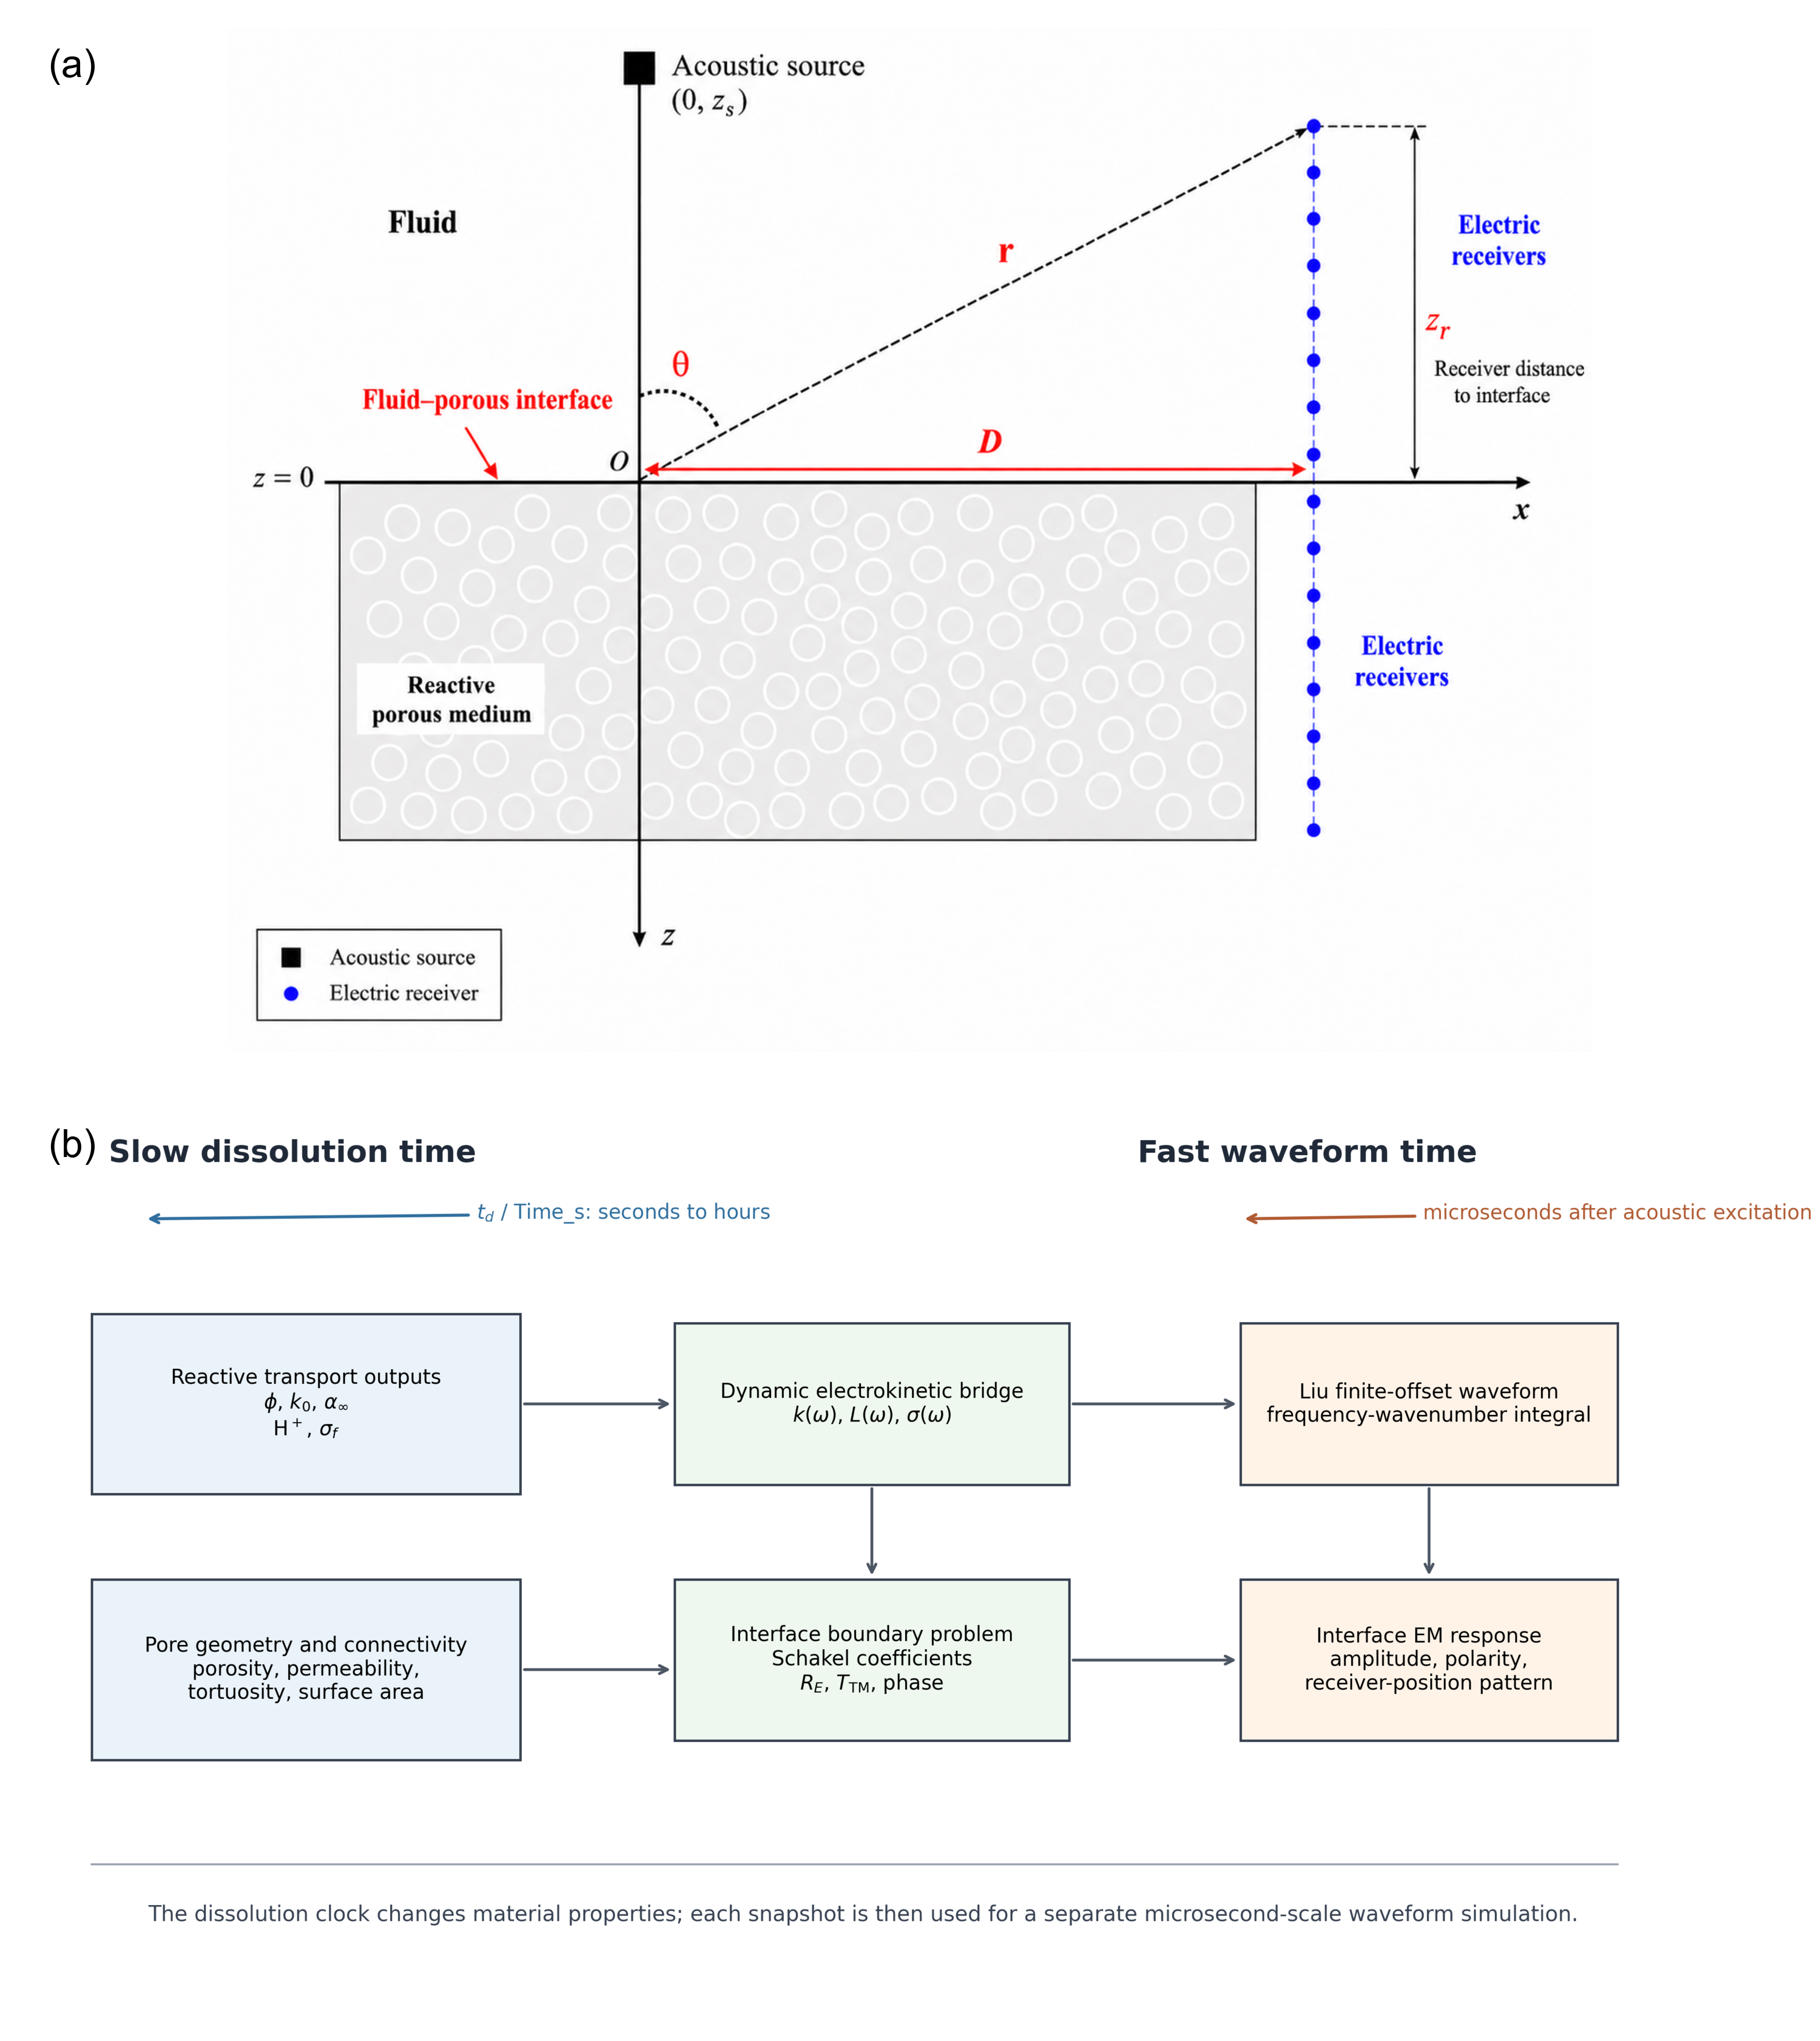
\includegraphics[width=\textwidth]{figures/figure1.png}
\caption{Finite-offset seismoelectric configuration and coupled modeling workflow. (a) Acoustic source, fluid-porous interface, offset distance, and electric receiver line used in the waveform synthesis. (b) Separation between dissolution time and waveform time, and the mapping from reactive transport outputs to dynamic electrokinetic properties, interface coefficients, and the interface electromagnetic response.}
\label{fig:workflow}
\end{figure}

\section{Model and Analysis Workflow}

\subsection{Reactive Transport Inputs}

We use three reactive transport simulations with Pe = 0.1, 1, and 10 as evolving porous media states.
For each time step, porosity, permeability, tortuosity, outlet $\mathrm{H}^+$ concentration, and derived pore-fluid conductivity define the material inputs to the seismoelectric model.

The analysis is restricted to the poroelastic validity window used in the current forward model.
This restriction keeps the interpretation focused on the part of dissolution evolution that can be mapped consistently into the Schakel/Pride-type seismoelectric formulation.

\subsection{Mapping Reactive Transport Outputs to Dynamic Electrokinetic Properties}

The reactive transport variables are converted into frequency-dependent permeability, dynamic electrokinetic coupling $L(\omega)$, and dynamic conductivity $\sigma(\omega)$.
This step defines the physical bridge between chemical evolution and the electromagnetic source terms used in the interface problem.

\subsection{Interface Conversion Coefficients}

For each evolved state, the dynamic properties are inserted into the fluid-porous medium interface boundary value problem.
The main coefficient-level quantities are the reflected electric response $R_E$ and transmitted transverse magnetic response $T_{\mathrm{TM}}$.

\subsection{Finite-Offset Waveform Synthesis}

Finite-offset waveforms are calculated with a frequency-wavenumber spectral integral following the Liu-type VSEP geometry.
Each waveform panel is indexed by dissolution time but plotted against waveform time after acoustic excitation.

\subsection{Numerical Diagnostics and Response Metrics}

The waveform synthesis is checked for pre-$T_0$ leakage and frequency sampling convergence.
Normalized $R_E$, $T_{\mathrm{TM}}$, $|L|/|\sigma|$, and spectral-ratio metrics are then used as simulation-based indicators of response change.

\section{Results}

\subsection{Dissolution Changes Hydraulic and Electrical Pathways Together}

Dissolution increases porosity and permeability in all Pe cases, but the permeability increase is much larger for Pe = 1 and Pe = 10 than for Pe = 0.1.
At the same time, the higher Pe cases develop much stronger pore-fluid conductivity growth, setting up the competition that controls the seismoelectric response.
Within the valid window, permeability increases by about 20 times for Pe = 0.1 and by more than 200 times for Pe = 1 and Pe = 10.

\begin{figure}
\noindent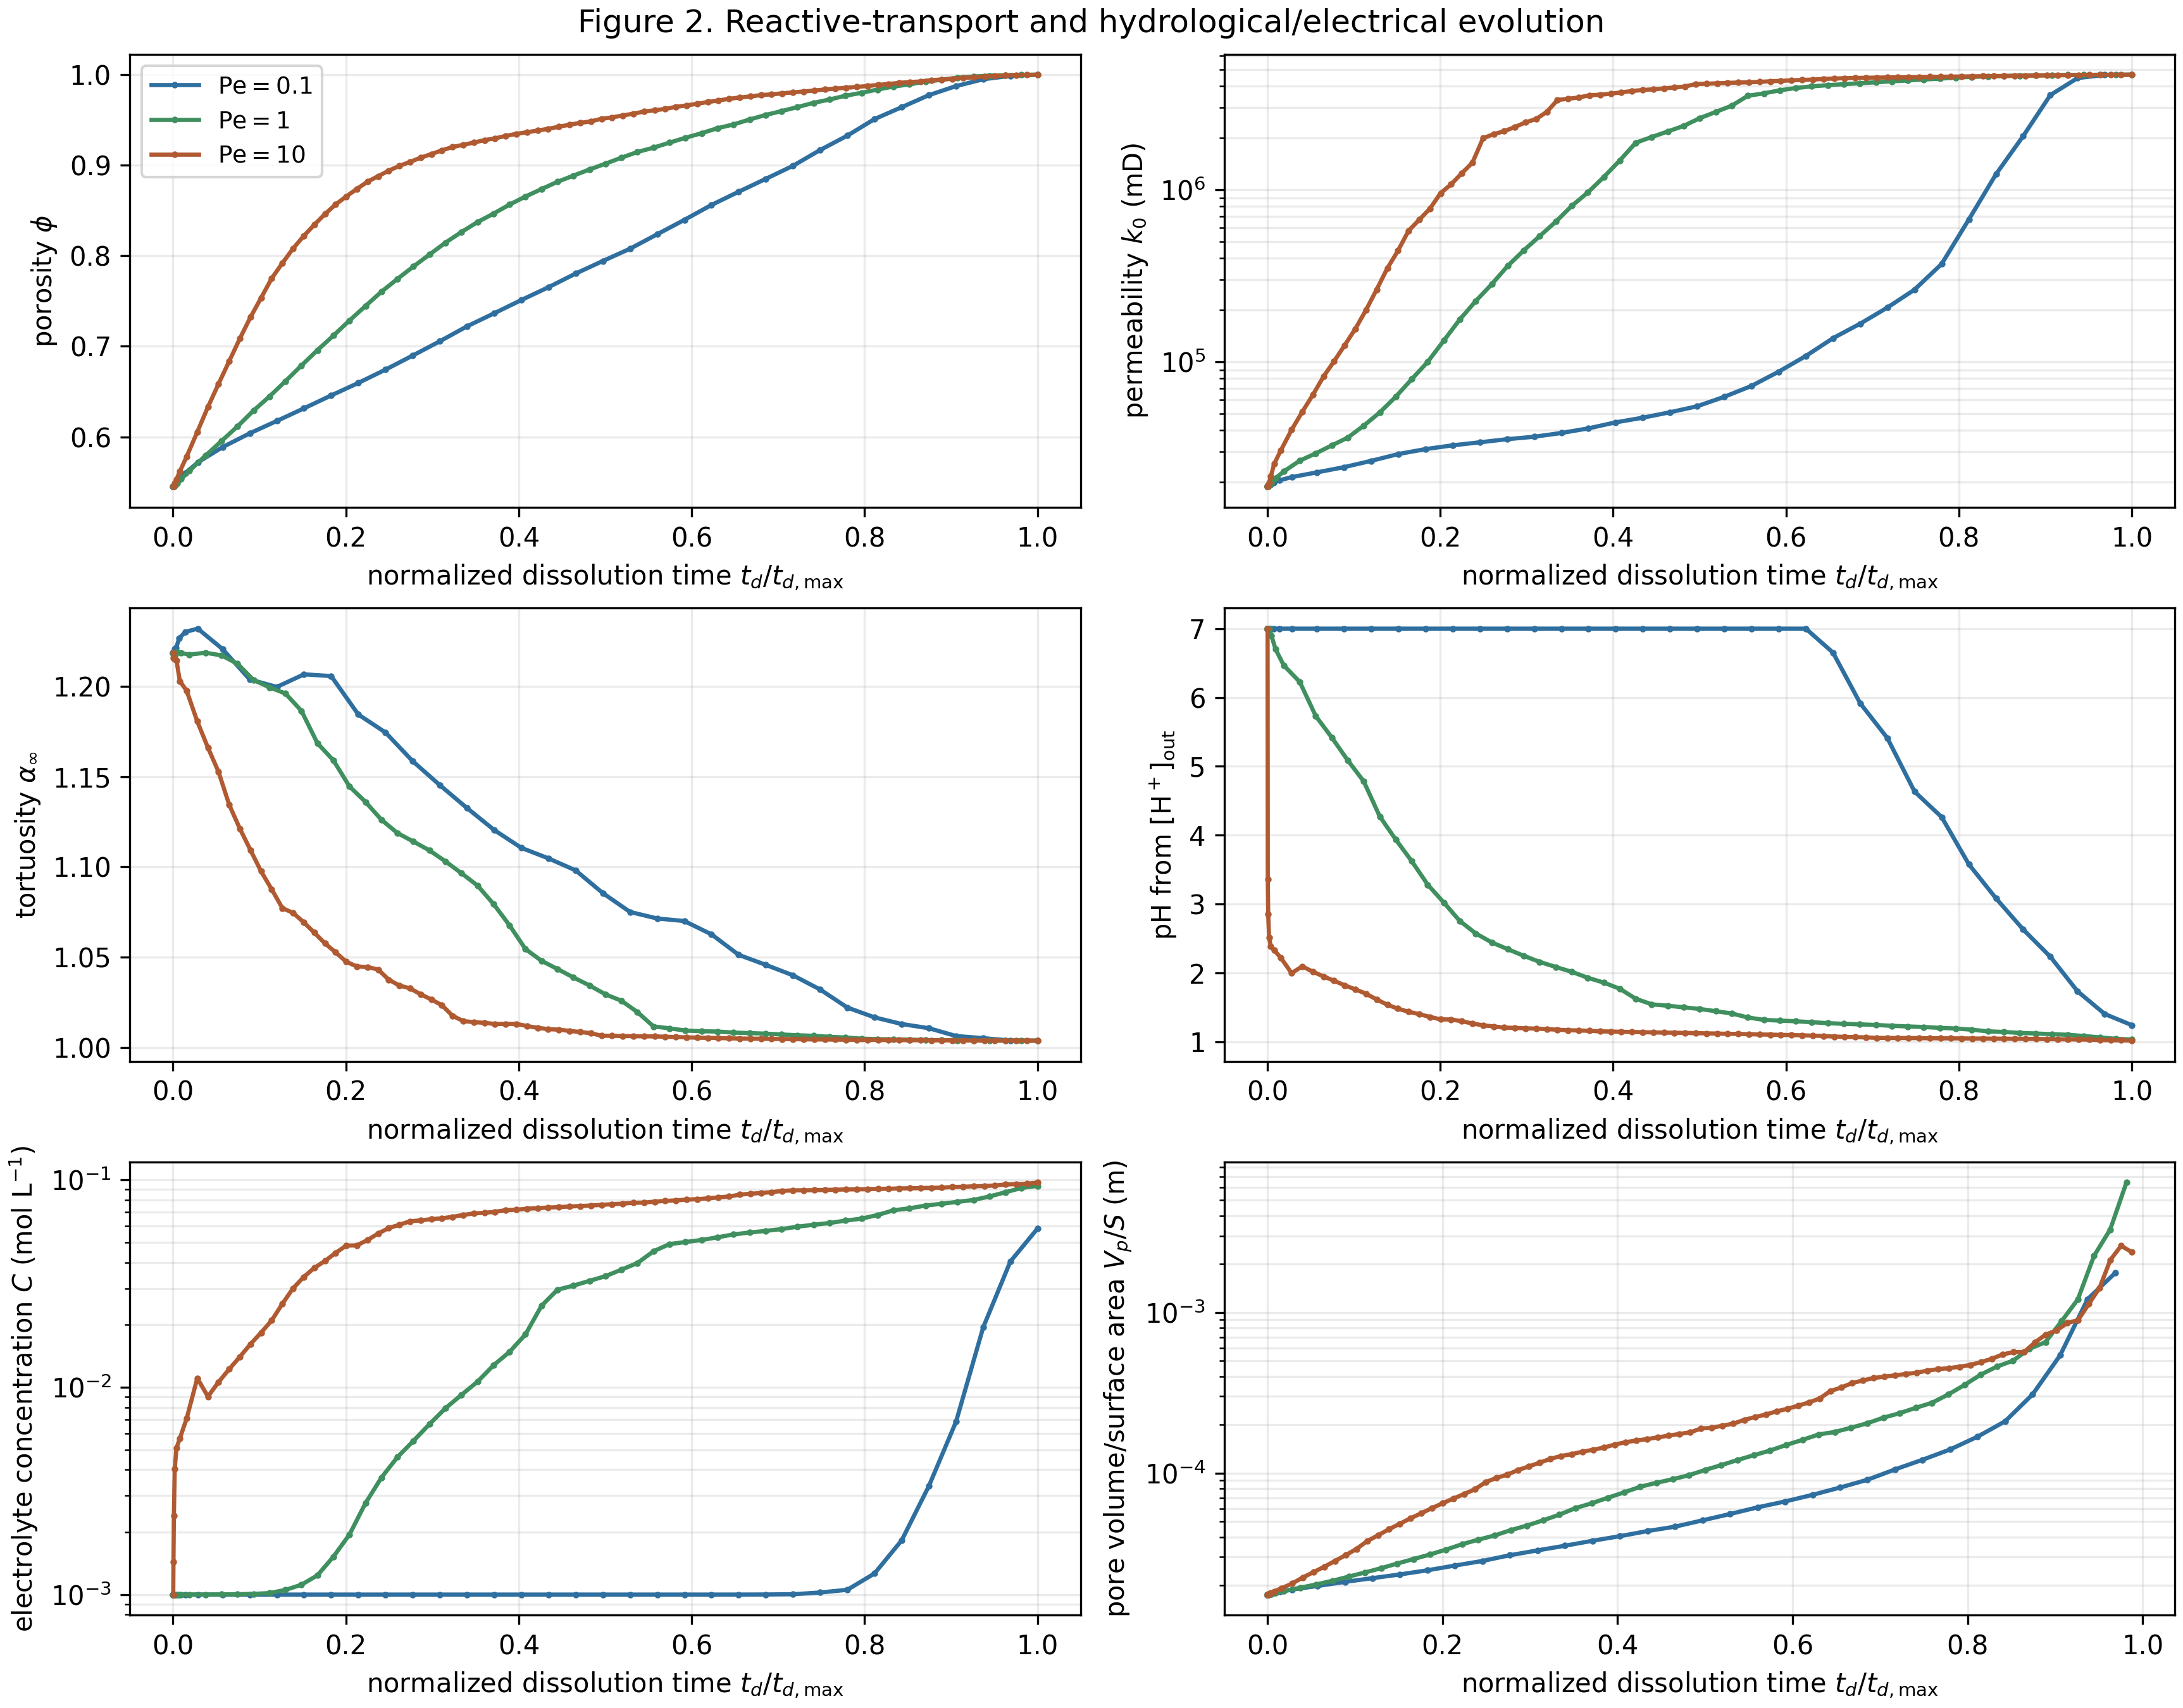
\includegraphics[width=\textwidth]{figures/figure2.png}
\caption{Reactive transport evolution of porosity, permeability, tortuosity, concentration, conductivity, and related state variables. The figure establishes the hydraulic and electrical pathways that feed the seismoelectric model.}
\label{fig:rt_evolution}
\end{figure}

\subsection{Dynamic Electrokinetic Properties Translate Dissolution Into Source Strength}

The dynamic bridge shows that $\sigma(\omega)$ increases with pore-fluid conductivity, whereas $L(\omega)$ decreases strongly in the higher Pe cases.
This result indicates that permeability alone is not a sufficient predictor of the interface electromagnetic response.
In Pe = 1 and Pe = 10, $|\sigma|$ increases by about 114--158 times, while $|L|$ decreases to about 1\% of its initial value.

\begin{figure}
\noindent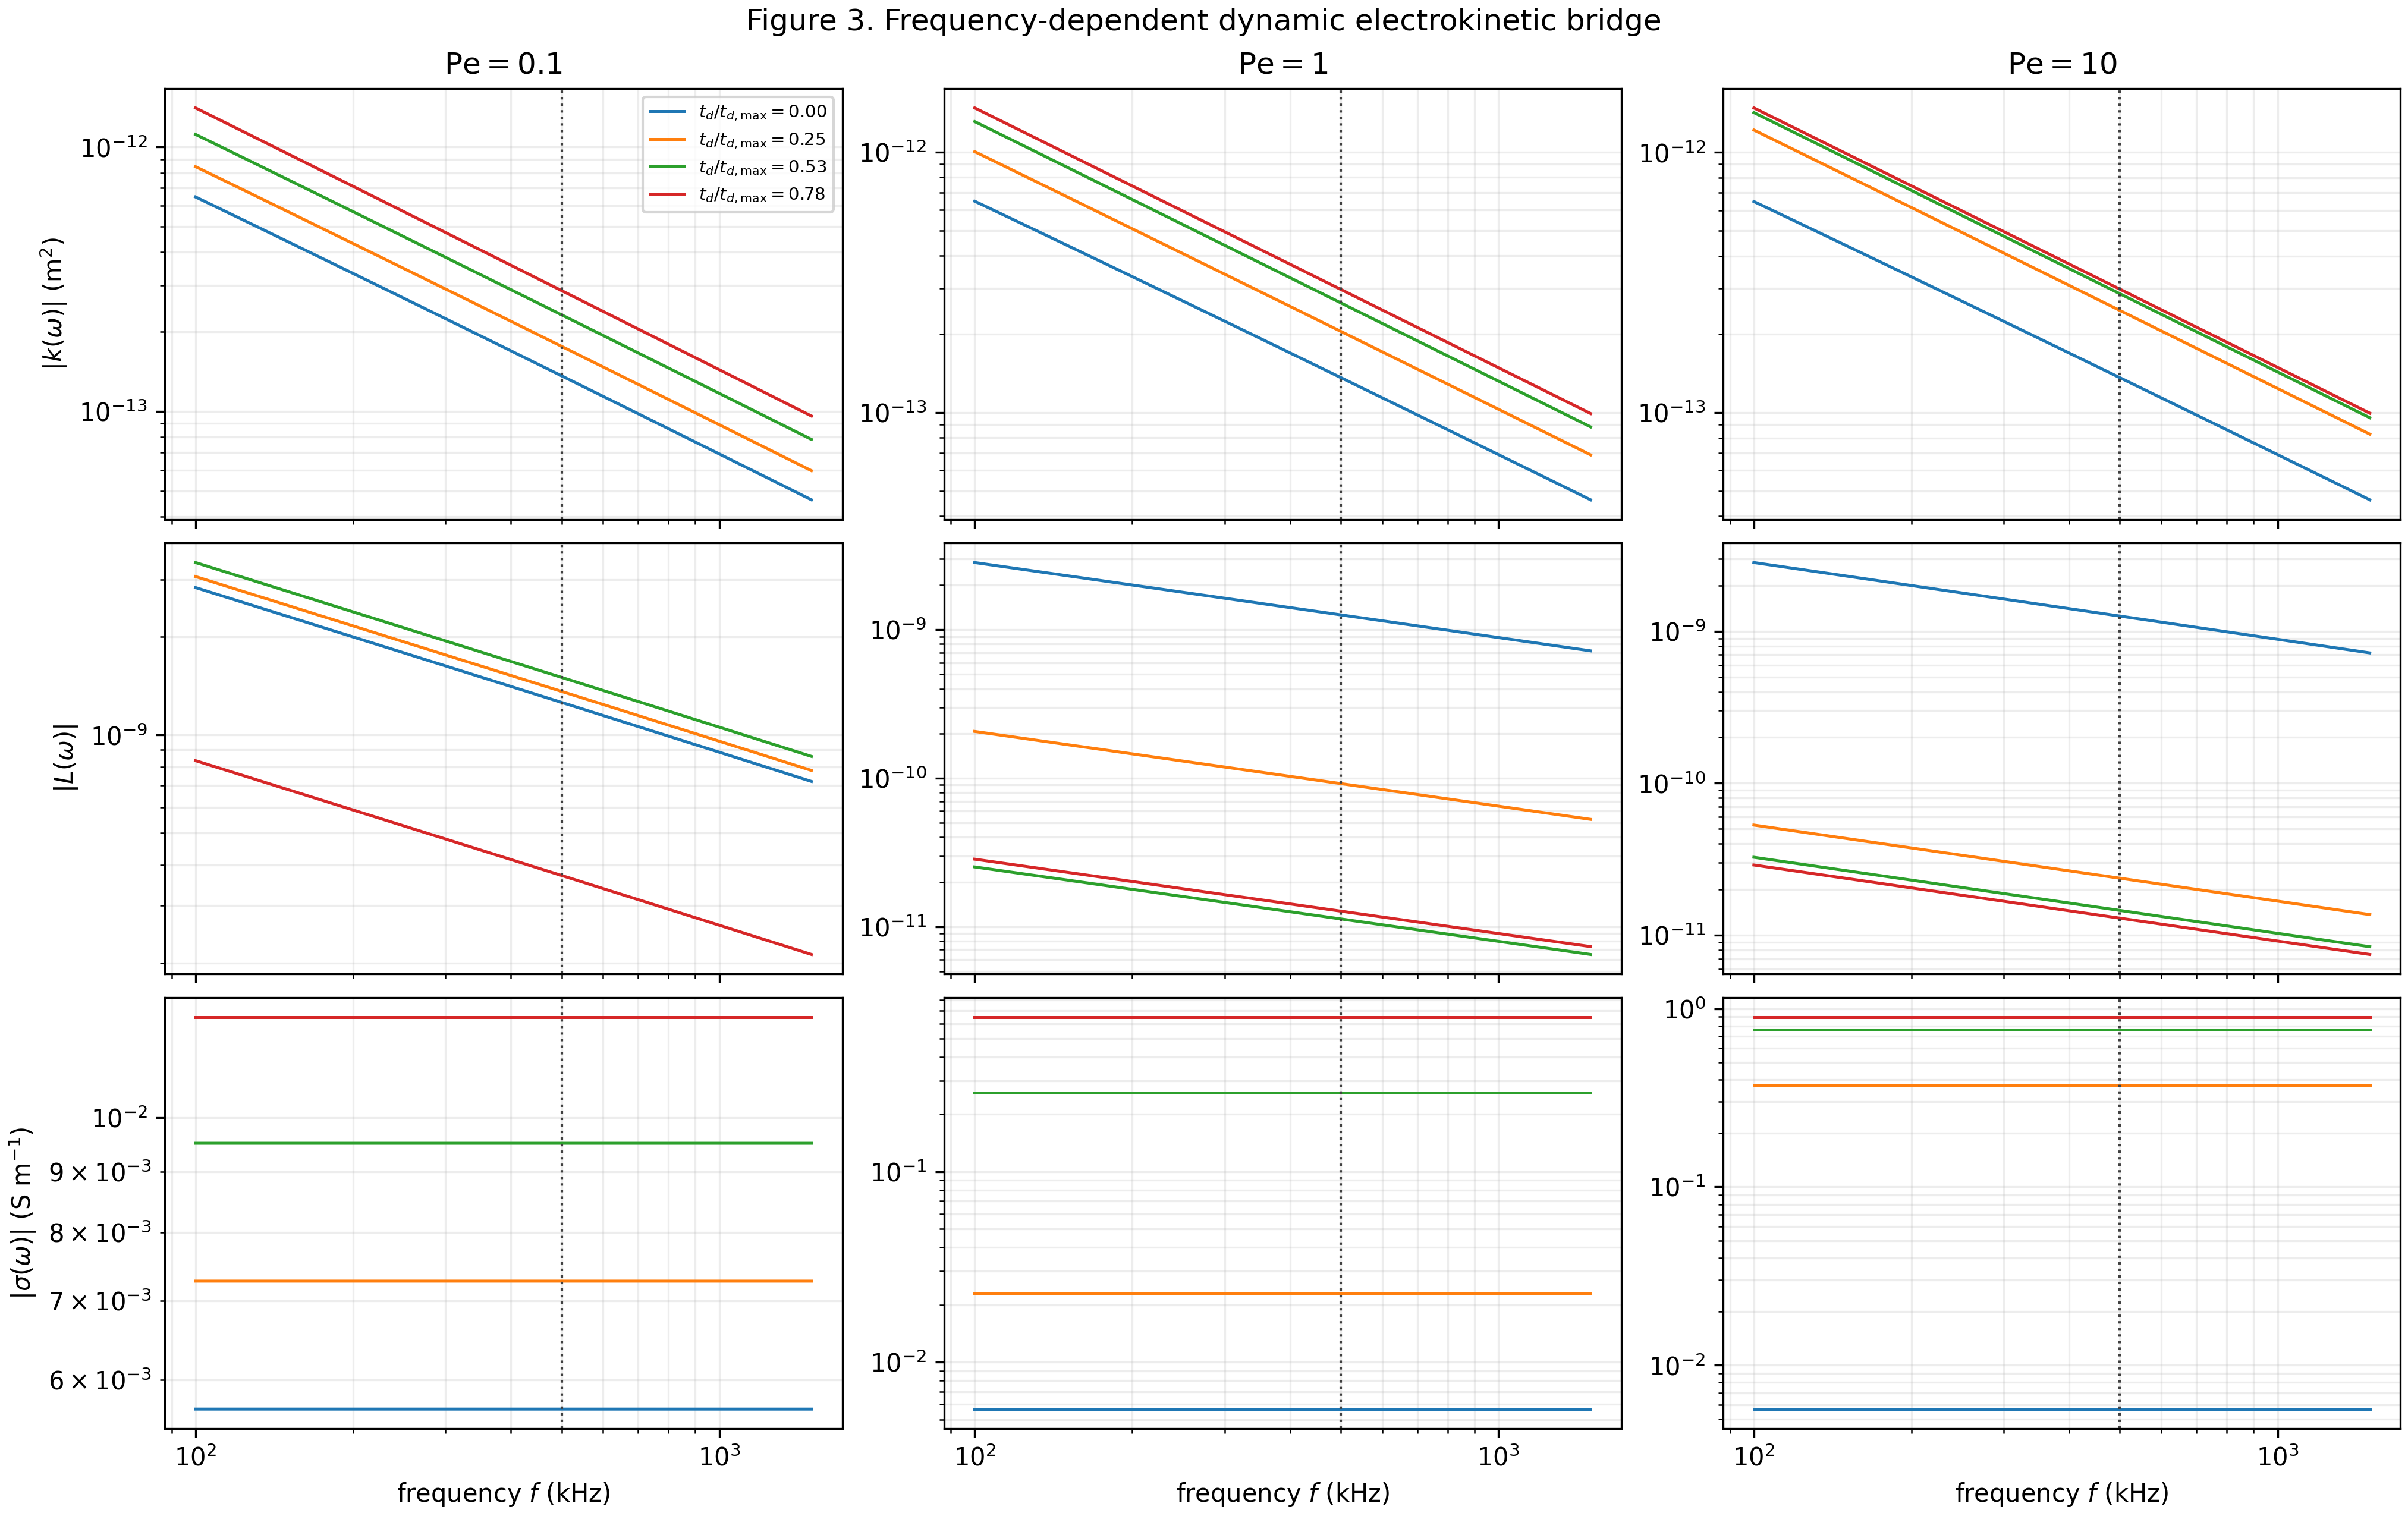
\includegraphics[width=\textwidth]{figures/figure3.png}
\caption{Frequency-dependent dynamic electrokinetic properties derived from the reactive transport states. The opposing trends in $L(\omega)$ and $\sigma(\omega)$ define the main source-strength competition.}
\label{fig:dynamic_bridge}
\end{figure}

\subsection{Interface Conversion Coefficients Record Conductivity-Controlled Weakening}

The magnitude of $R_E$ decreases moderately for Pe = 0.1 but falls by nearly four orders of magnitude for Pe = 1 and Pe = 10 within the valid window.
Frequency-angle heatmaps show that this weakening persists across the sampled incident-wave and frequency space.
This contrast indicates that conductivity growth can outweigh the effect of increased hydraulic connectivity in the interface coefficients.

\begin{figure}
\noindent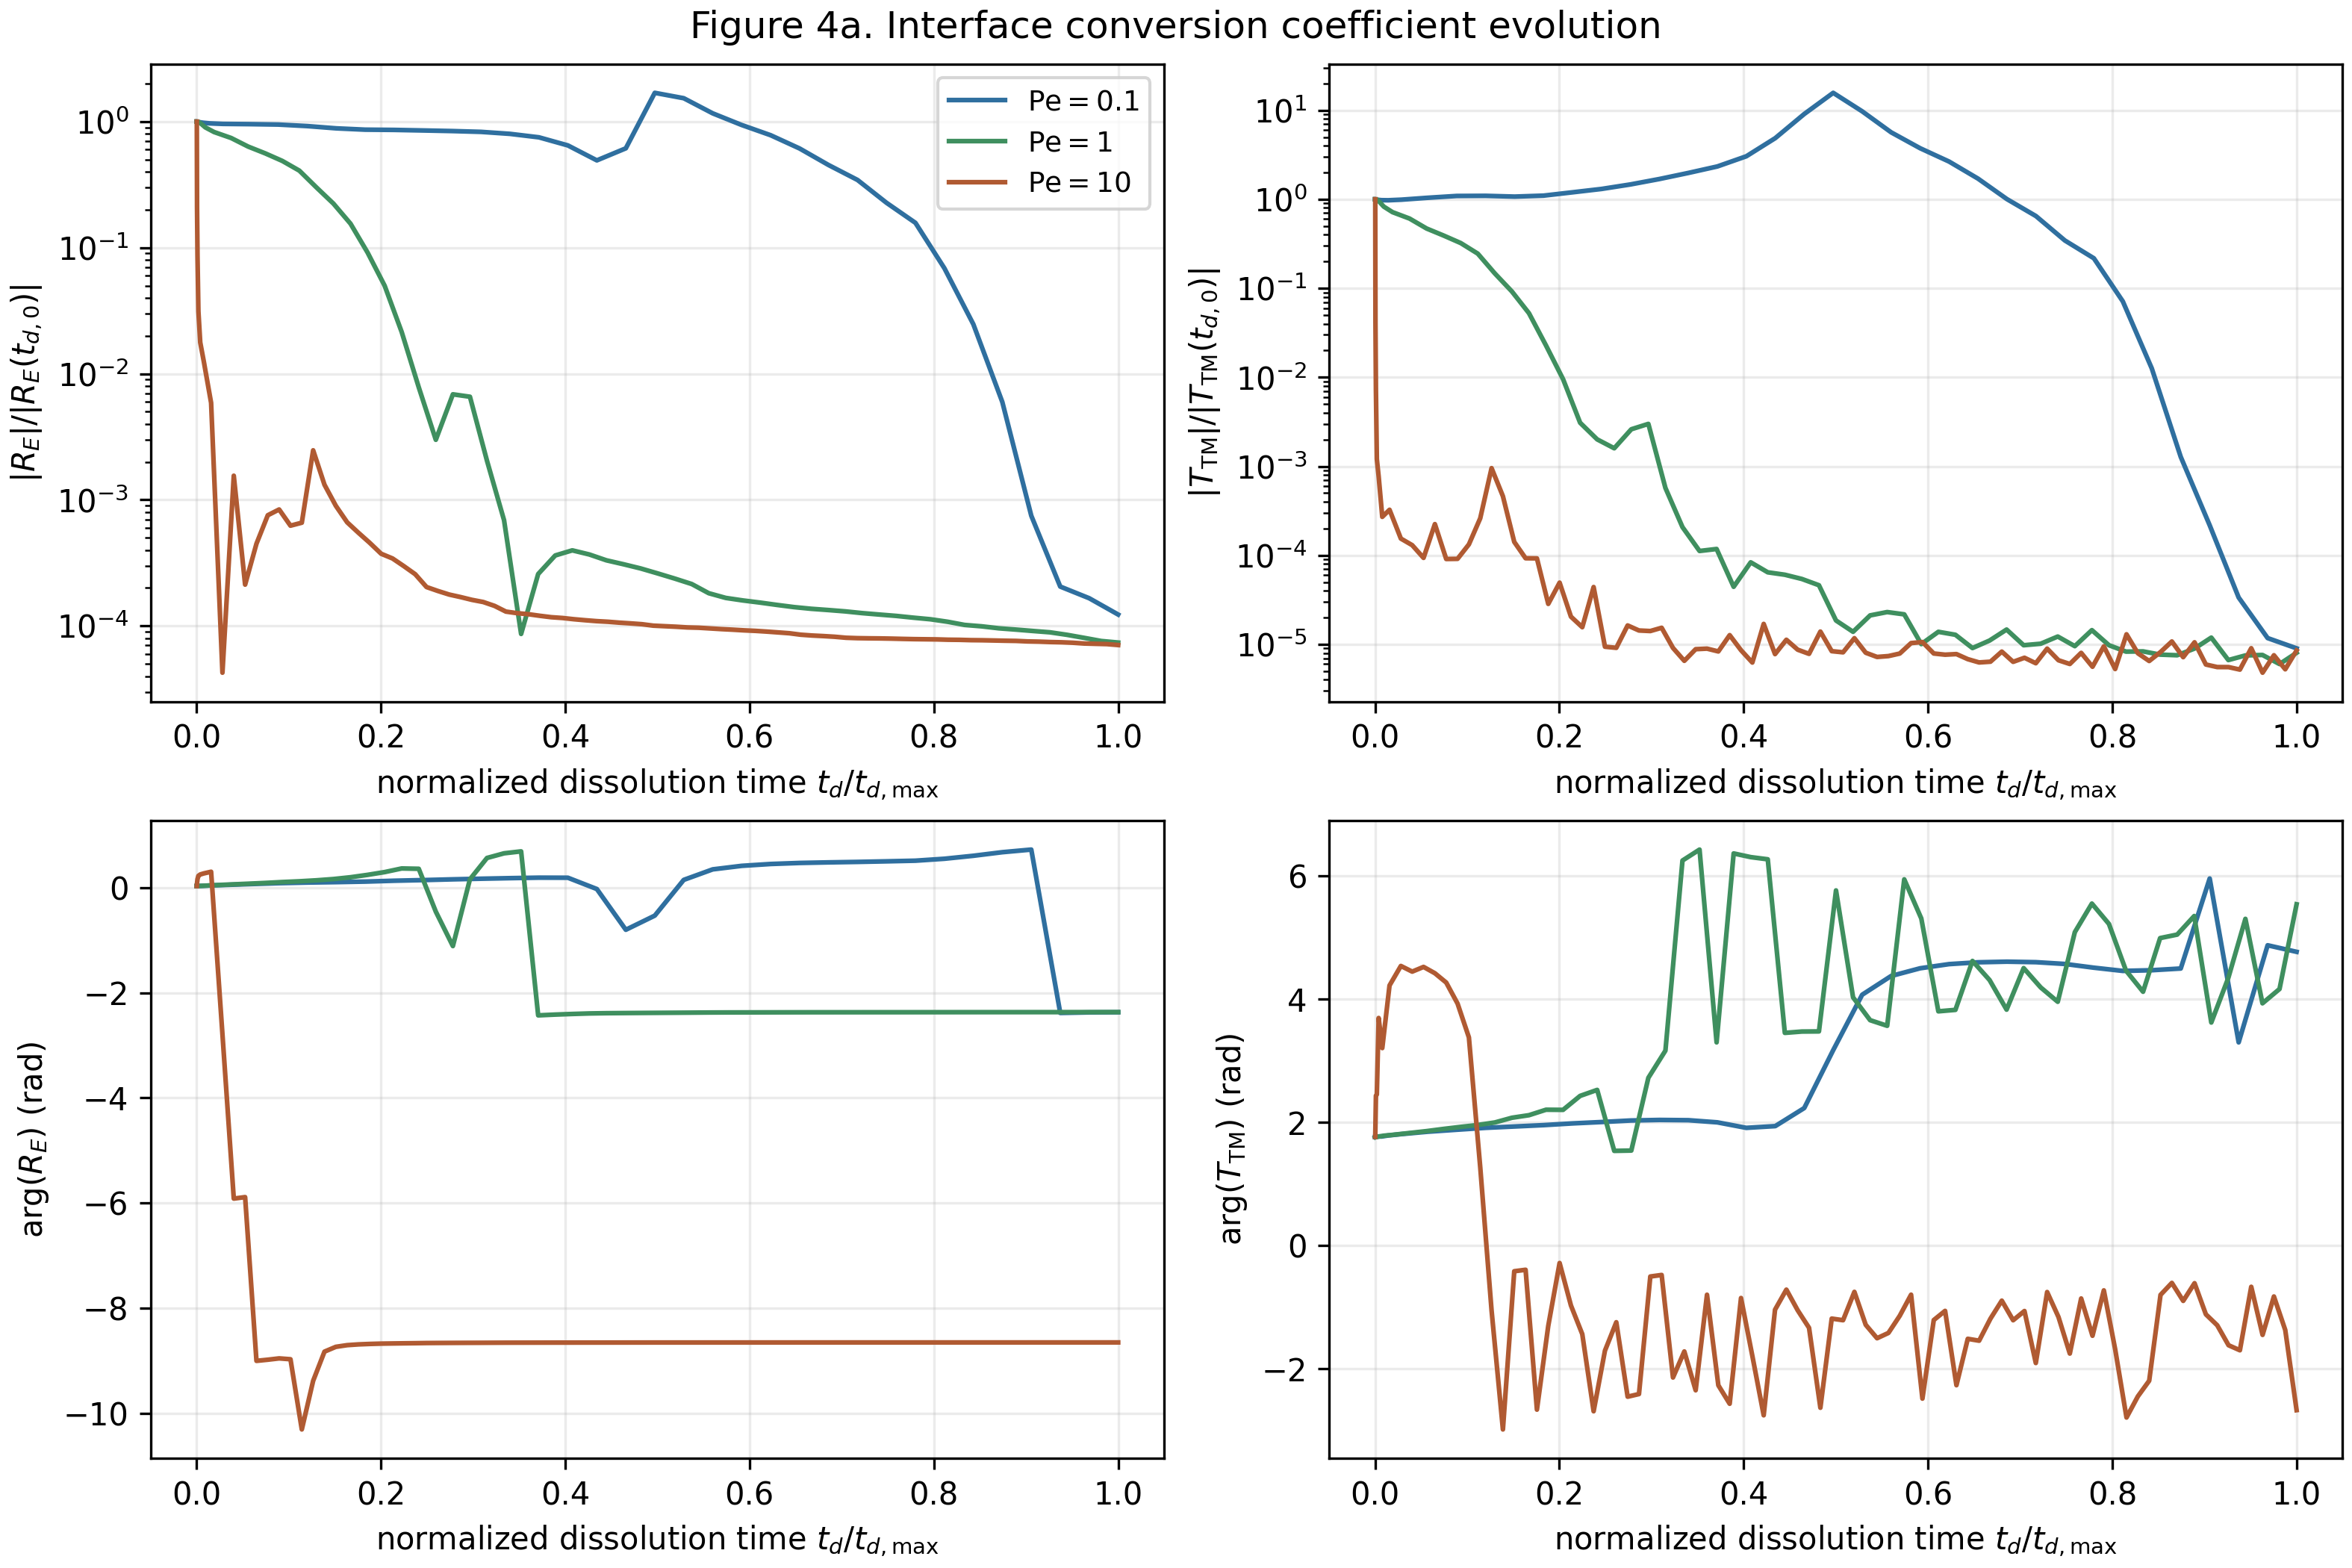
\includegraphics[width=\textwidth]{figures/figure4a.png}
\vspace{0.5em}
\noindent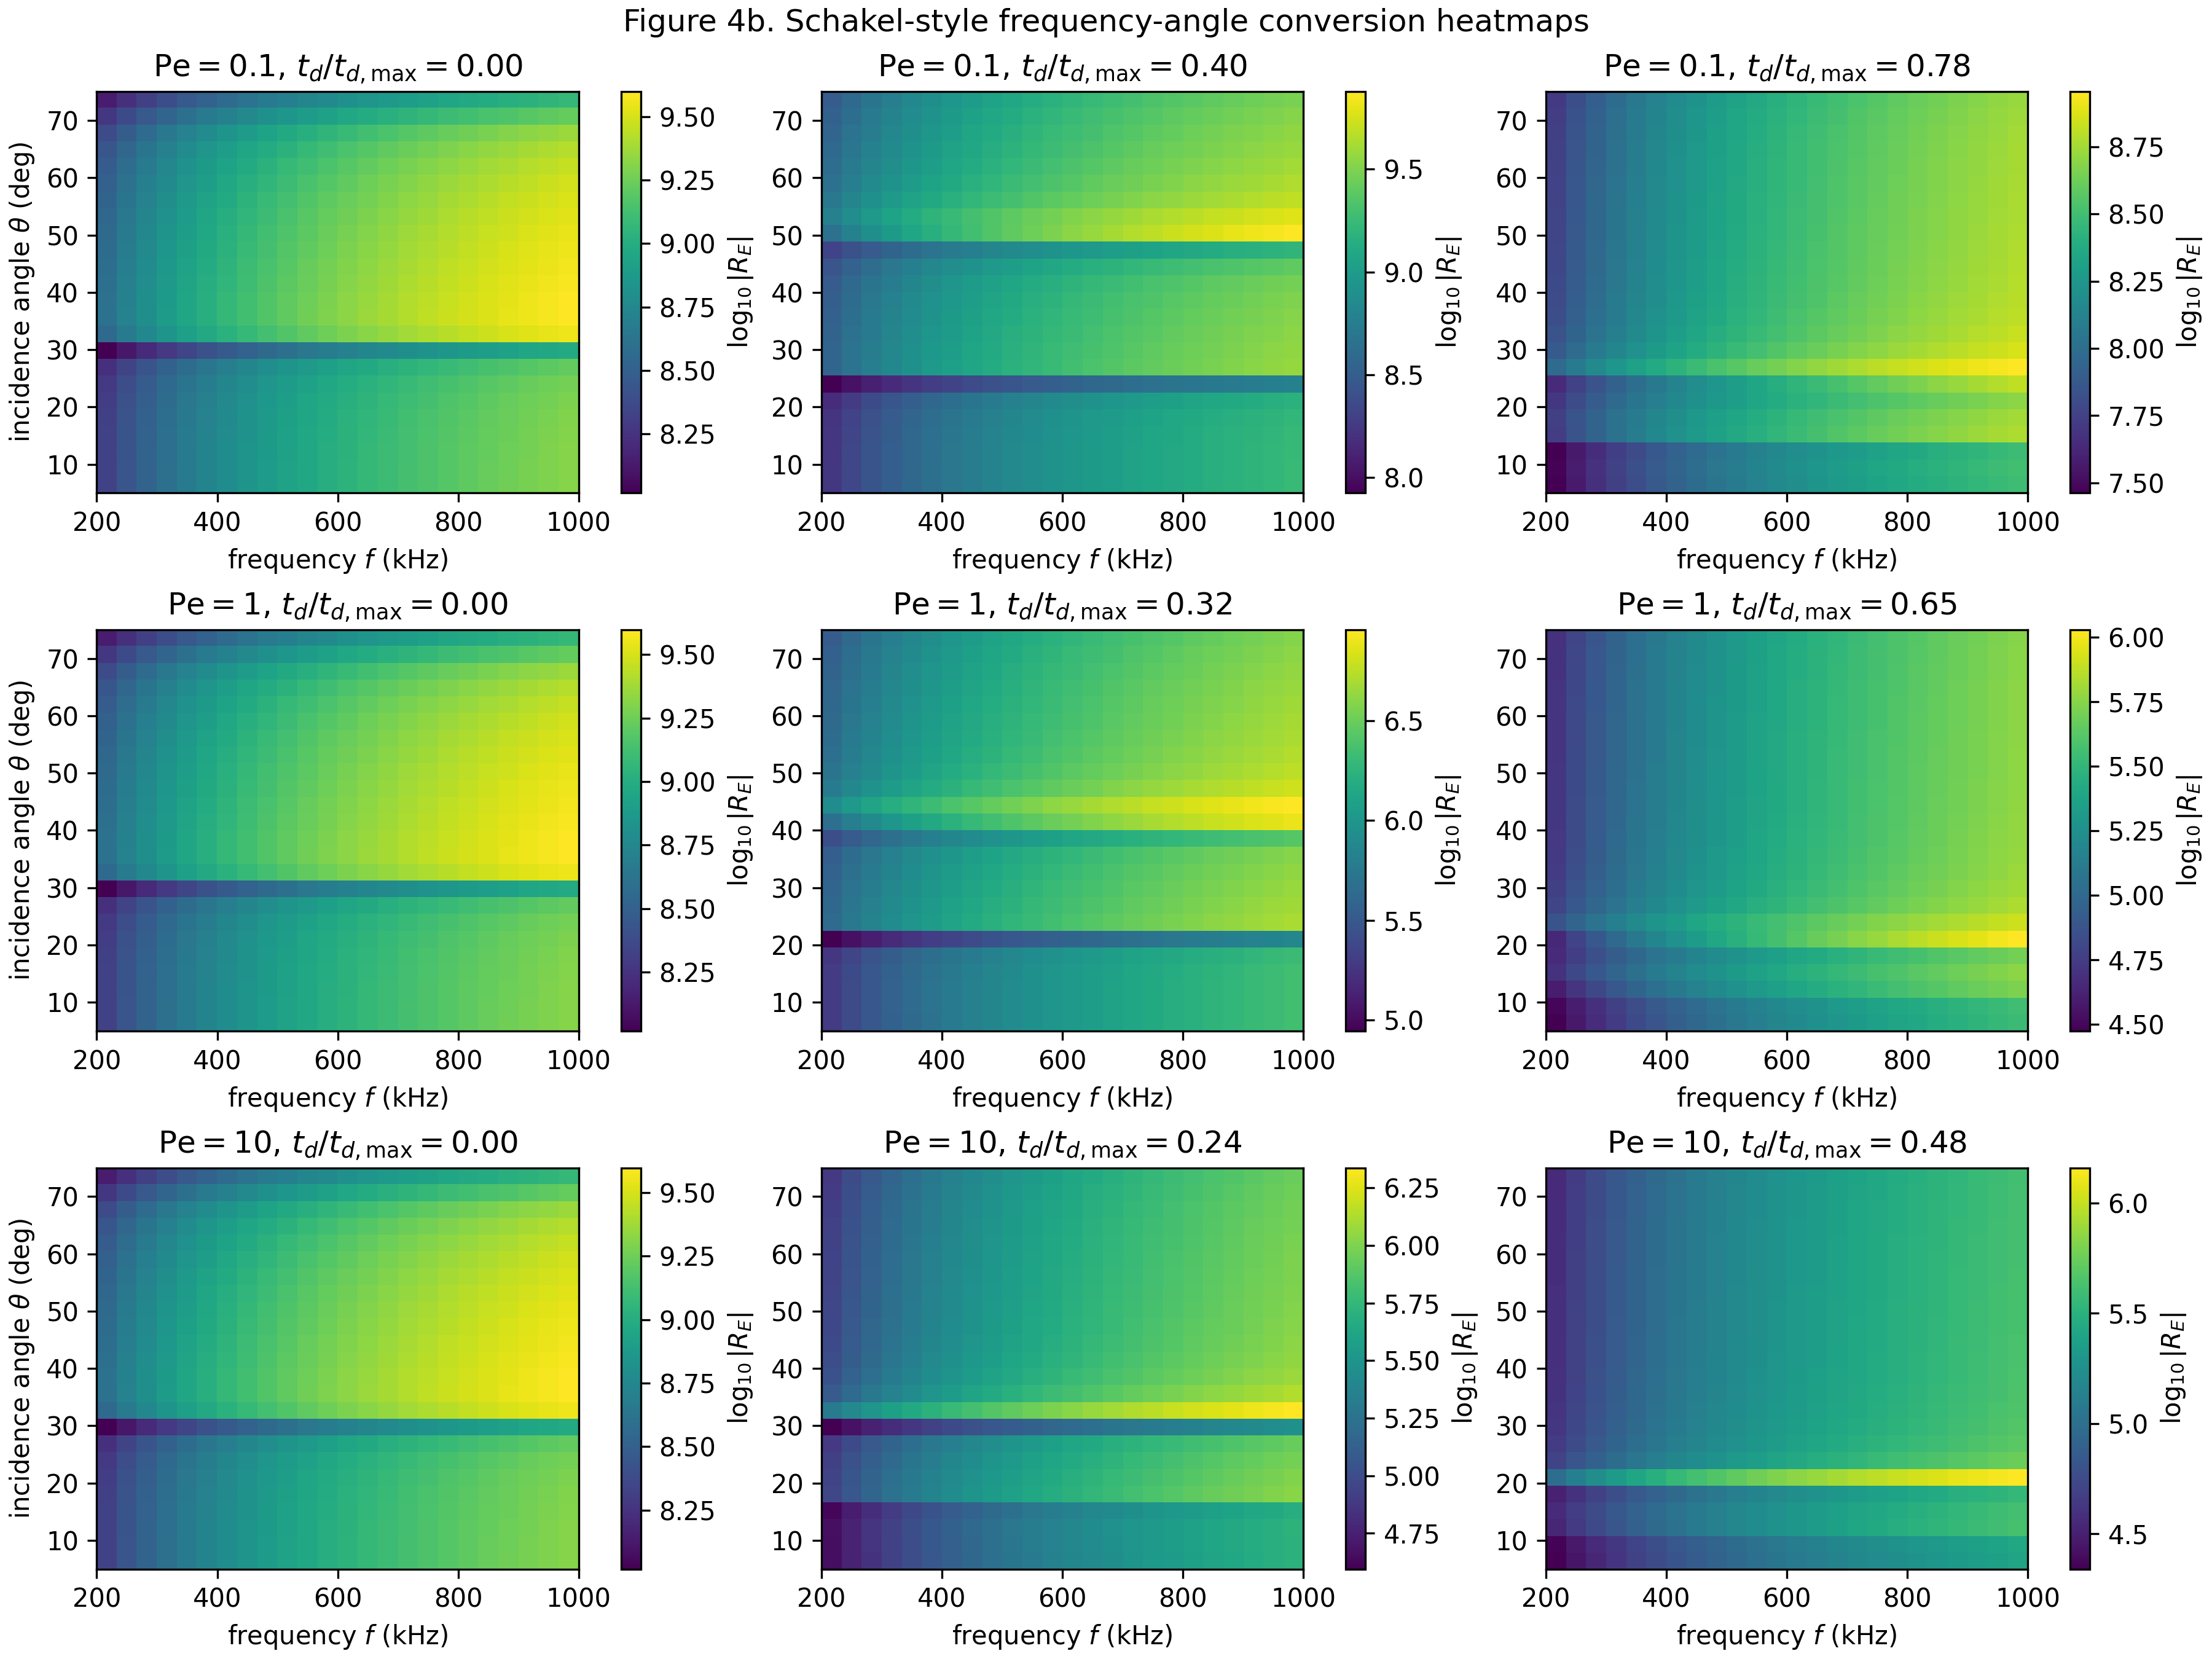
\includegraphics[width=\textwidth]{figures/figure4b.png}
\caption{Interface conversion coefficients during dissolution. The time series show how dynamic property changes are transferred into conversion strength, and the frequency-angle heatmaps separate wavefield dependence from the dissolution trend.}
\label{fig:conversion}
\end{figure}

\subsection{Finite-Offset Waveforms Preserve the Same Weakening in Waveform Time}

The post-$T_0$ finite-offset response weakens as dissolution proceeds, with the strongest amplitude loss in Pe = 1 and Pe = 10.
The waveform result therefore carries the coefficient-level suppression into the time-domain waveform response in the simulations.
Late-stage post-$T_0$ peaks are about $1.6\times10^{15}$ for Pe = 0.1, compared with about $1.8\times10^{12}$ for Pe = 1 and $1.3\times10^{12}$ for Pe = 10.

\begin{figure}
\noindent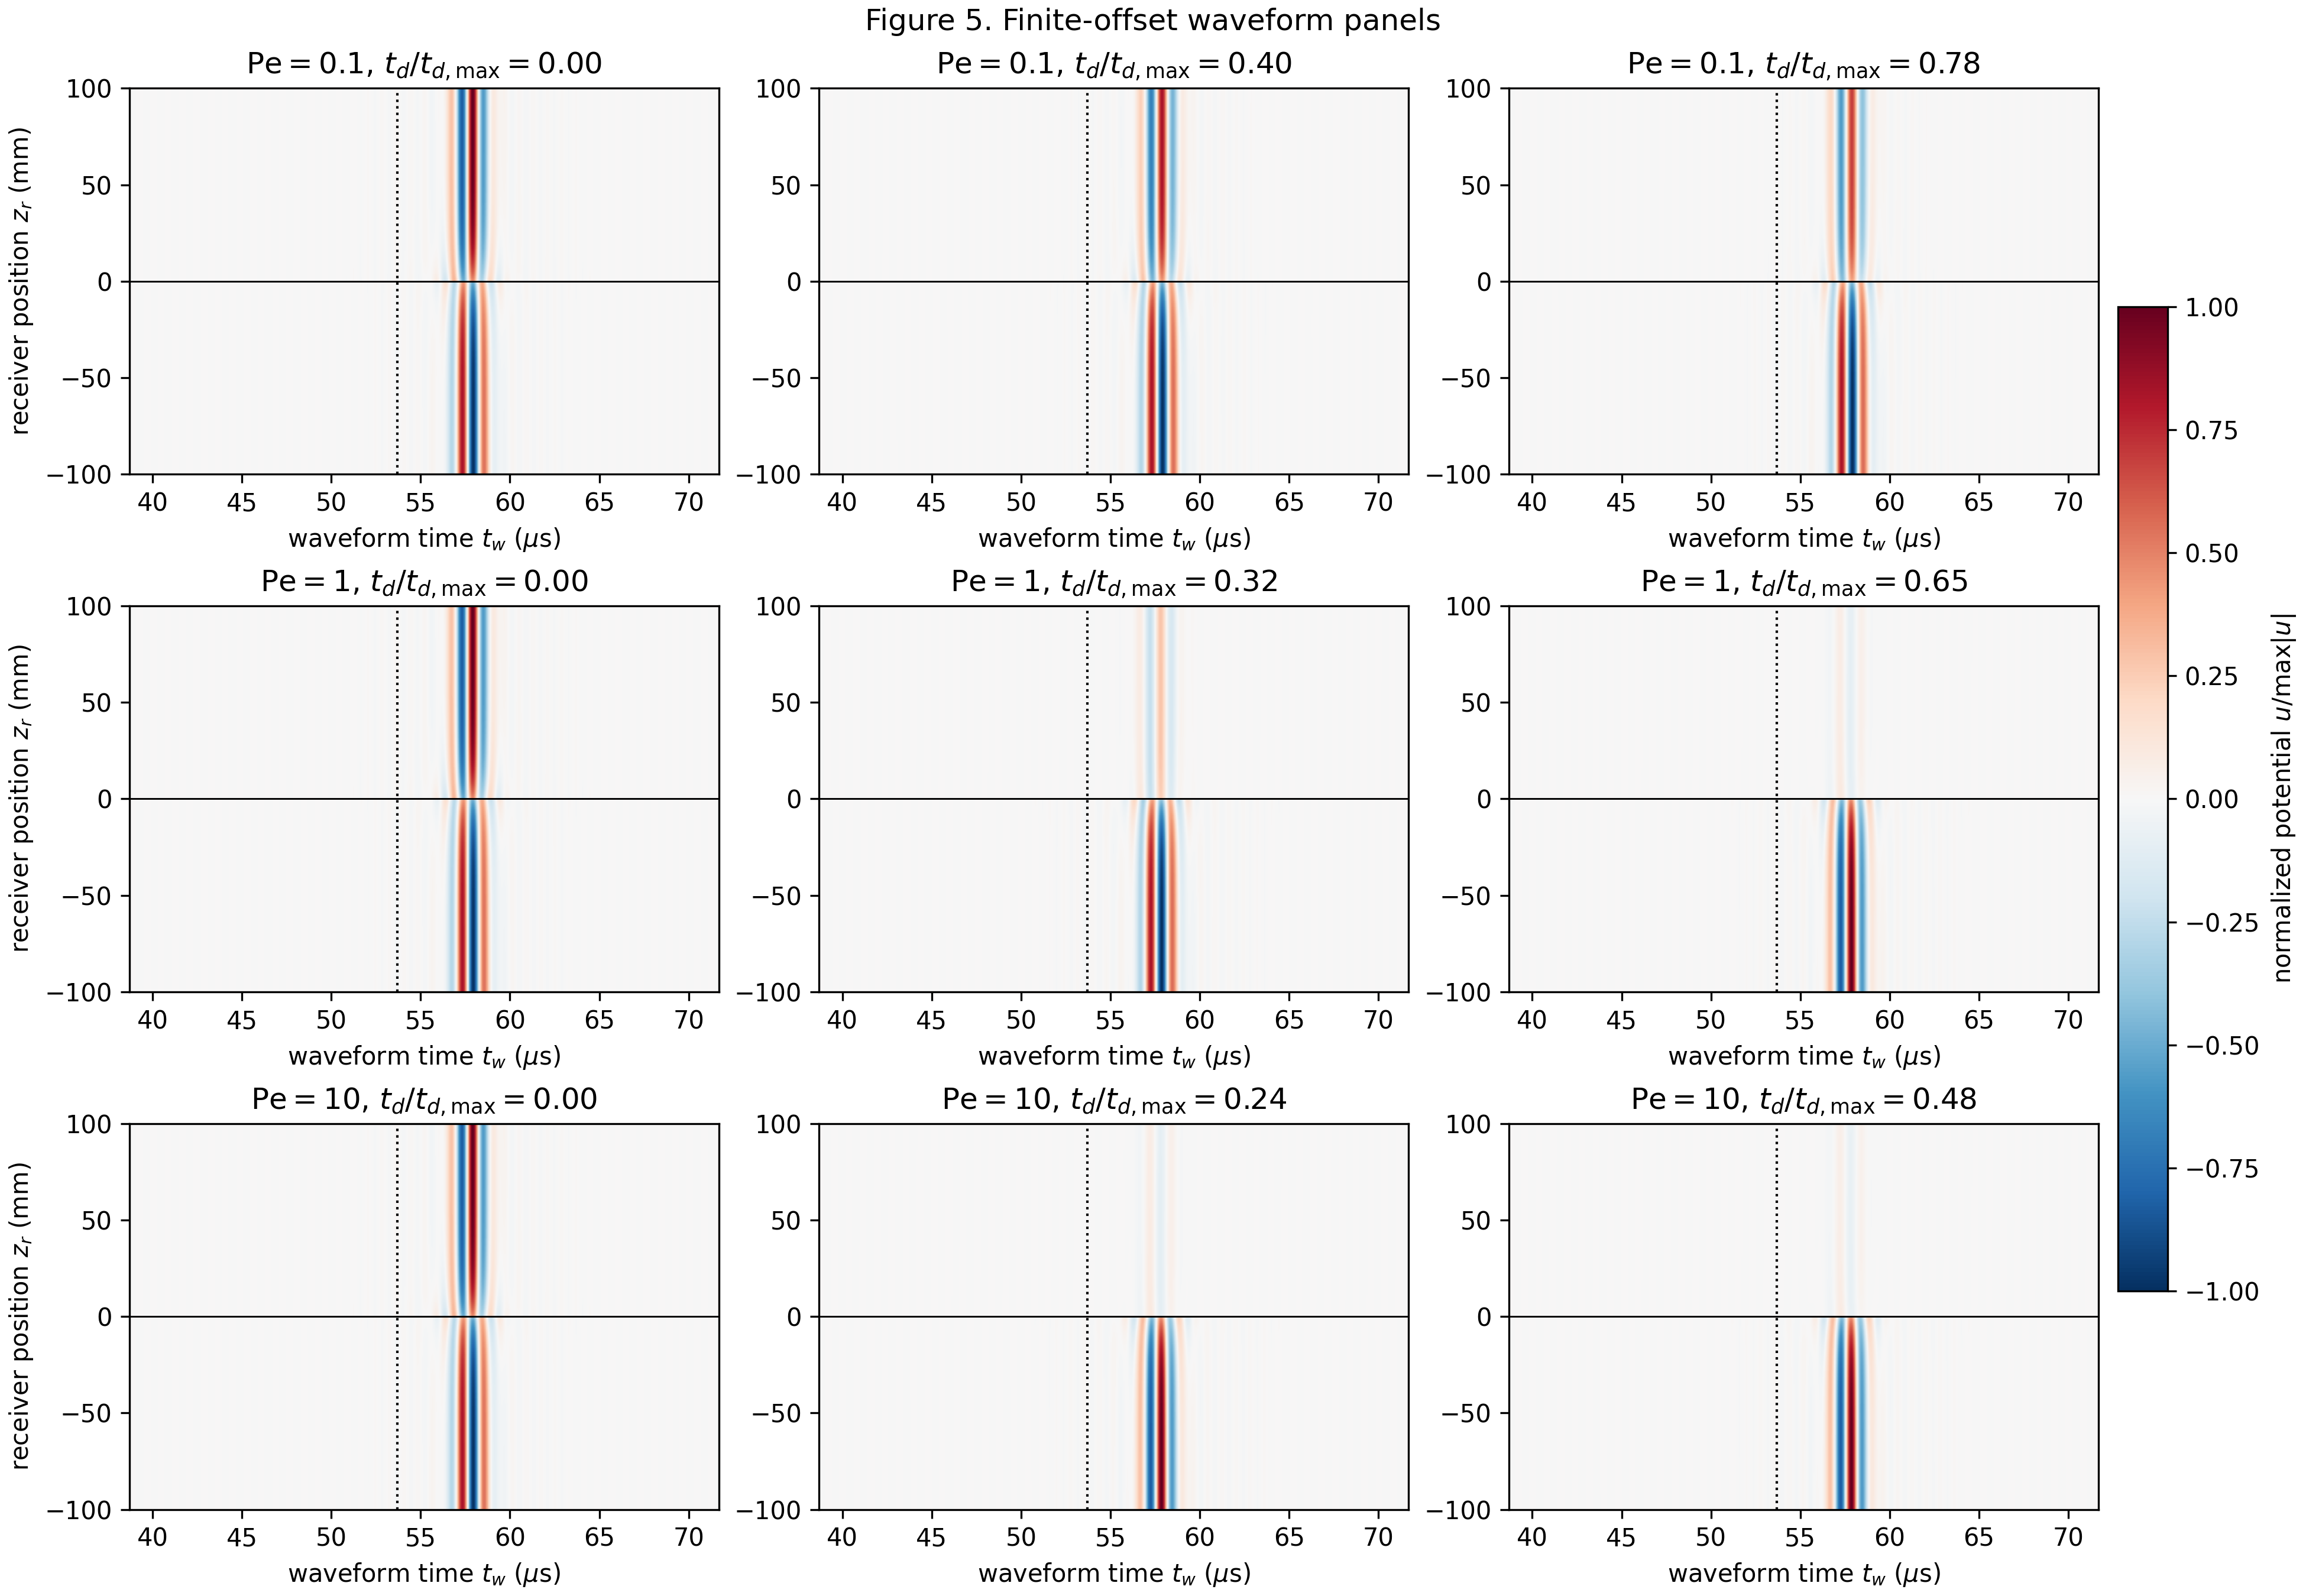
\includegraphics[width=\textwidth]{figures/figure5.png}
\caption{Finite-offset waveform panels for selected dissolution states. Dissolution time indexes the material state, while waveform time records the response after acoustic excitation.}
\label{fig:waveforms}
\end{figure}

\subsection{Waveform Diagnostics Support the Post-$T_0$ Interpretation}

Frequency sampling tests show that coarse sampling can create pre-$T_0$ aliases, but using $n_\omega=128$ reduces the pre/post-$T_0$ ratio to about 0.011--0.012 across the waveform panels.
This diagnostic supports the interpretation that the plotted main response is not dominated by pre-arrival numerical leakage.
% Suggested Supporting Information figures: waveform_t0_leakage_diagnostics.png and waveform_frequency_convergence.png.

\subsection{Spatial Peak Patterns Are Consistent With an Interface Source Geometry}

The finite-offset peak amplitudes vary with receiver position and show polarity differences across the interface.
The Liu-type dipole pattern is used only as a normalized spatial interpretation, not as an additional multiplier on the forward waveform.
This subsection functions as a geometry consistency check before the mechanism decomposition.

\begin{figure}
\noindent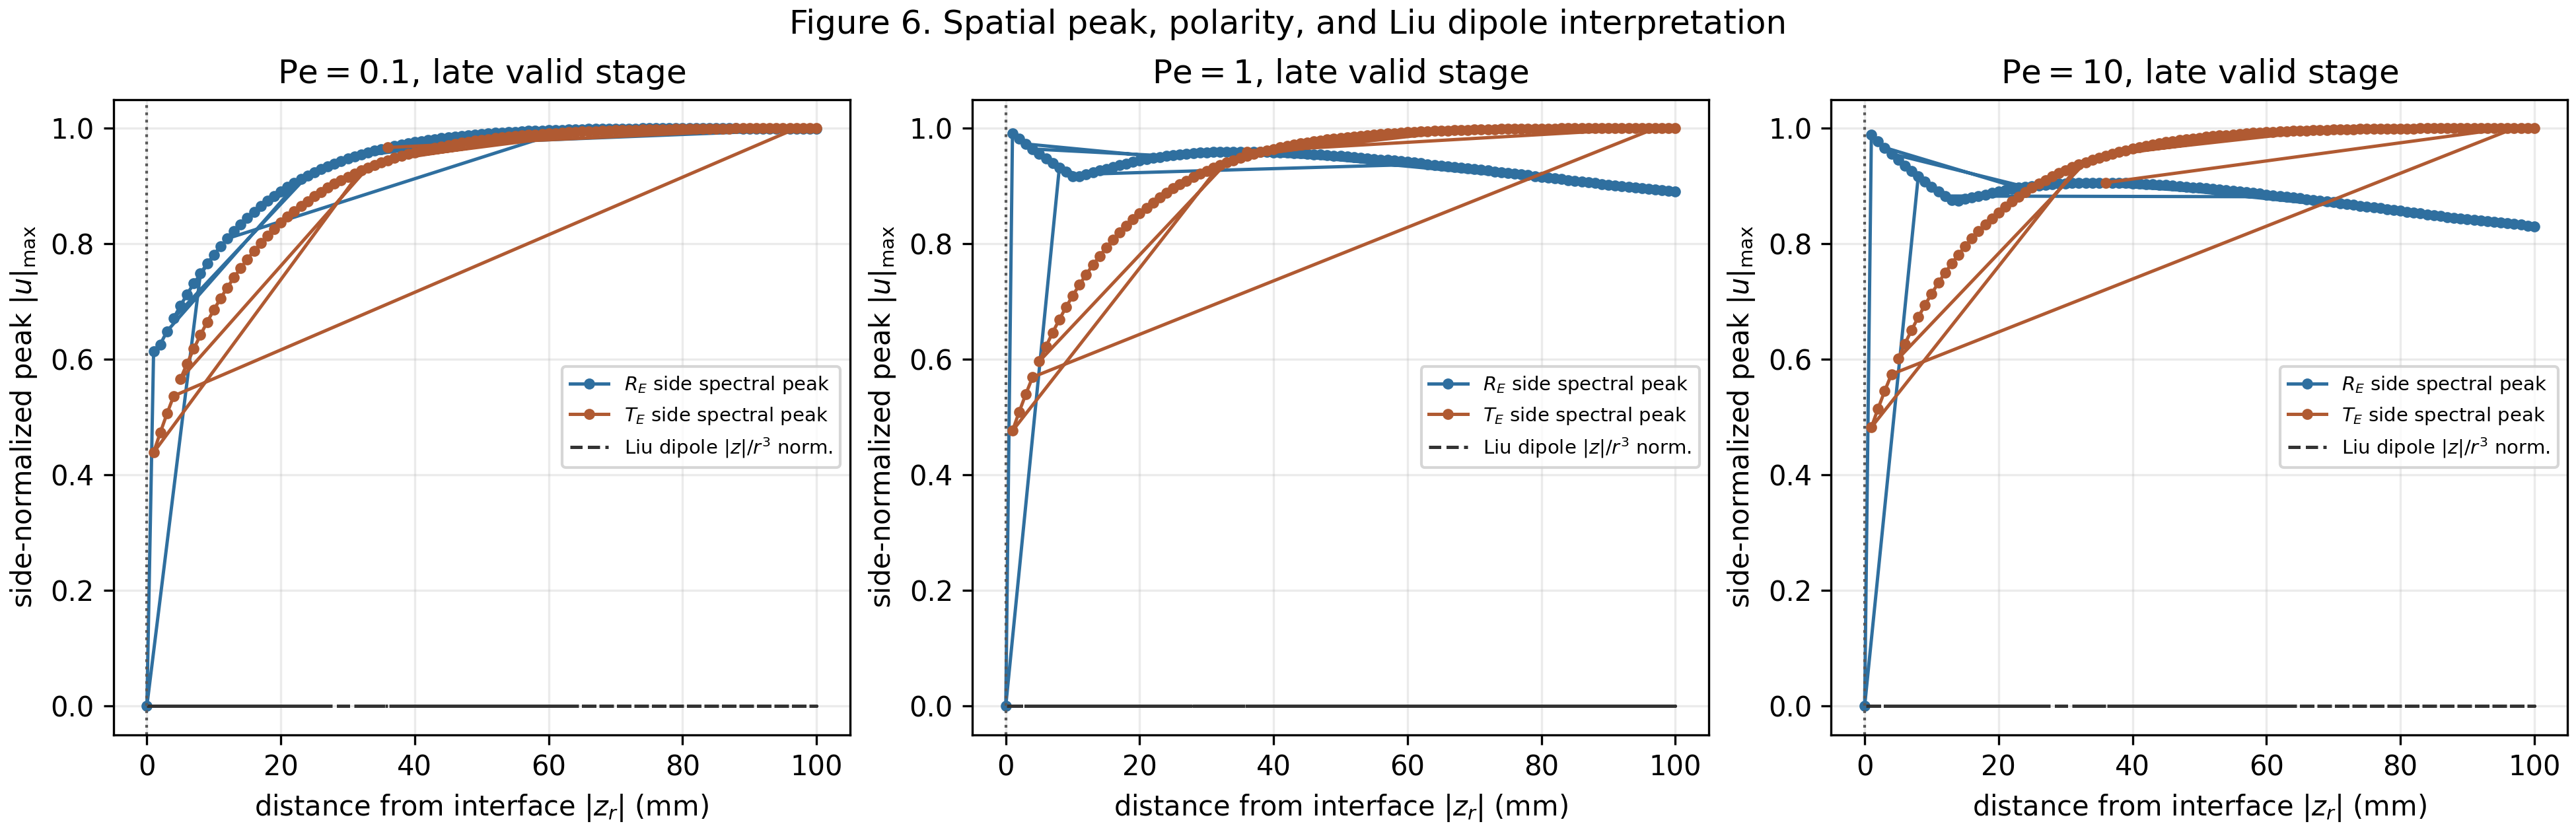
\includegraphics[width=\textwidth]{figures/figure6.png}
\caption{Spatial peak distribution, polarity behavior, and normalized dipole interpretation. The figure tests whether the modeled response has the expected finite-offset spatial organization.}
\label{fig:spatial_peak}
\end{figure}

\subsection{Mechanism Decomposition Identifies the Dominant Parameter Pathway}

One-at-a-time substitutions show that the largest negative contribution in Pe = 1 and Pe = 10 comes from the fluid chemistry pathway.
The late-stage amplitude loss is therefore interpreted mainly as conductivity-related weakening of electrokinetic coupling, with permeability and nonlinear interactions acting as secondary controls in the tested configuration.
For Pe = 1 and Pe = 10, the fluid chemistry pathway contributes log$_{10}$ peak changes of about -2.78 and -2.91, respectively.

\begin{figure}
\noindent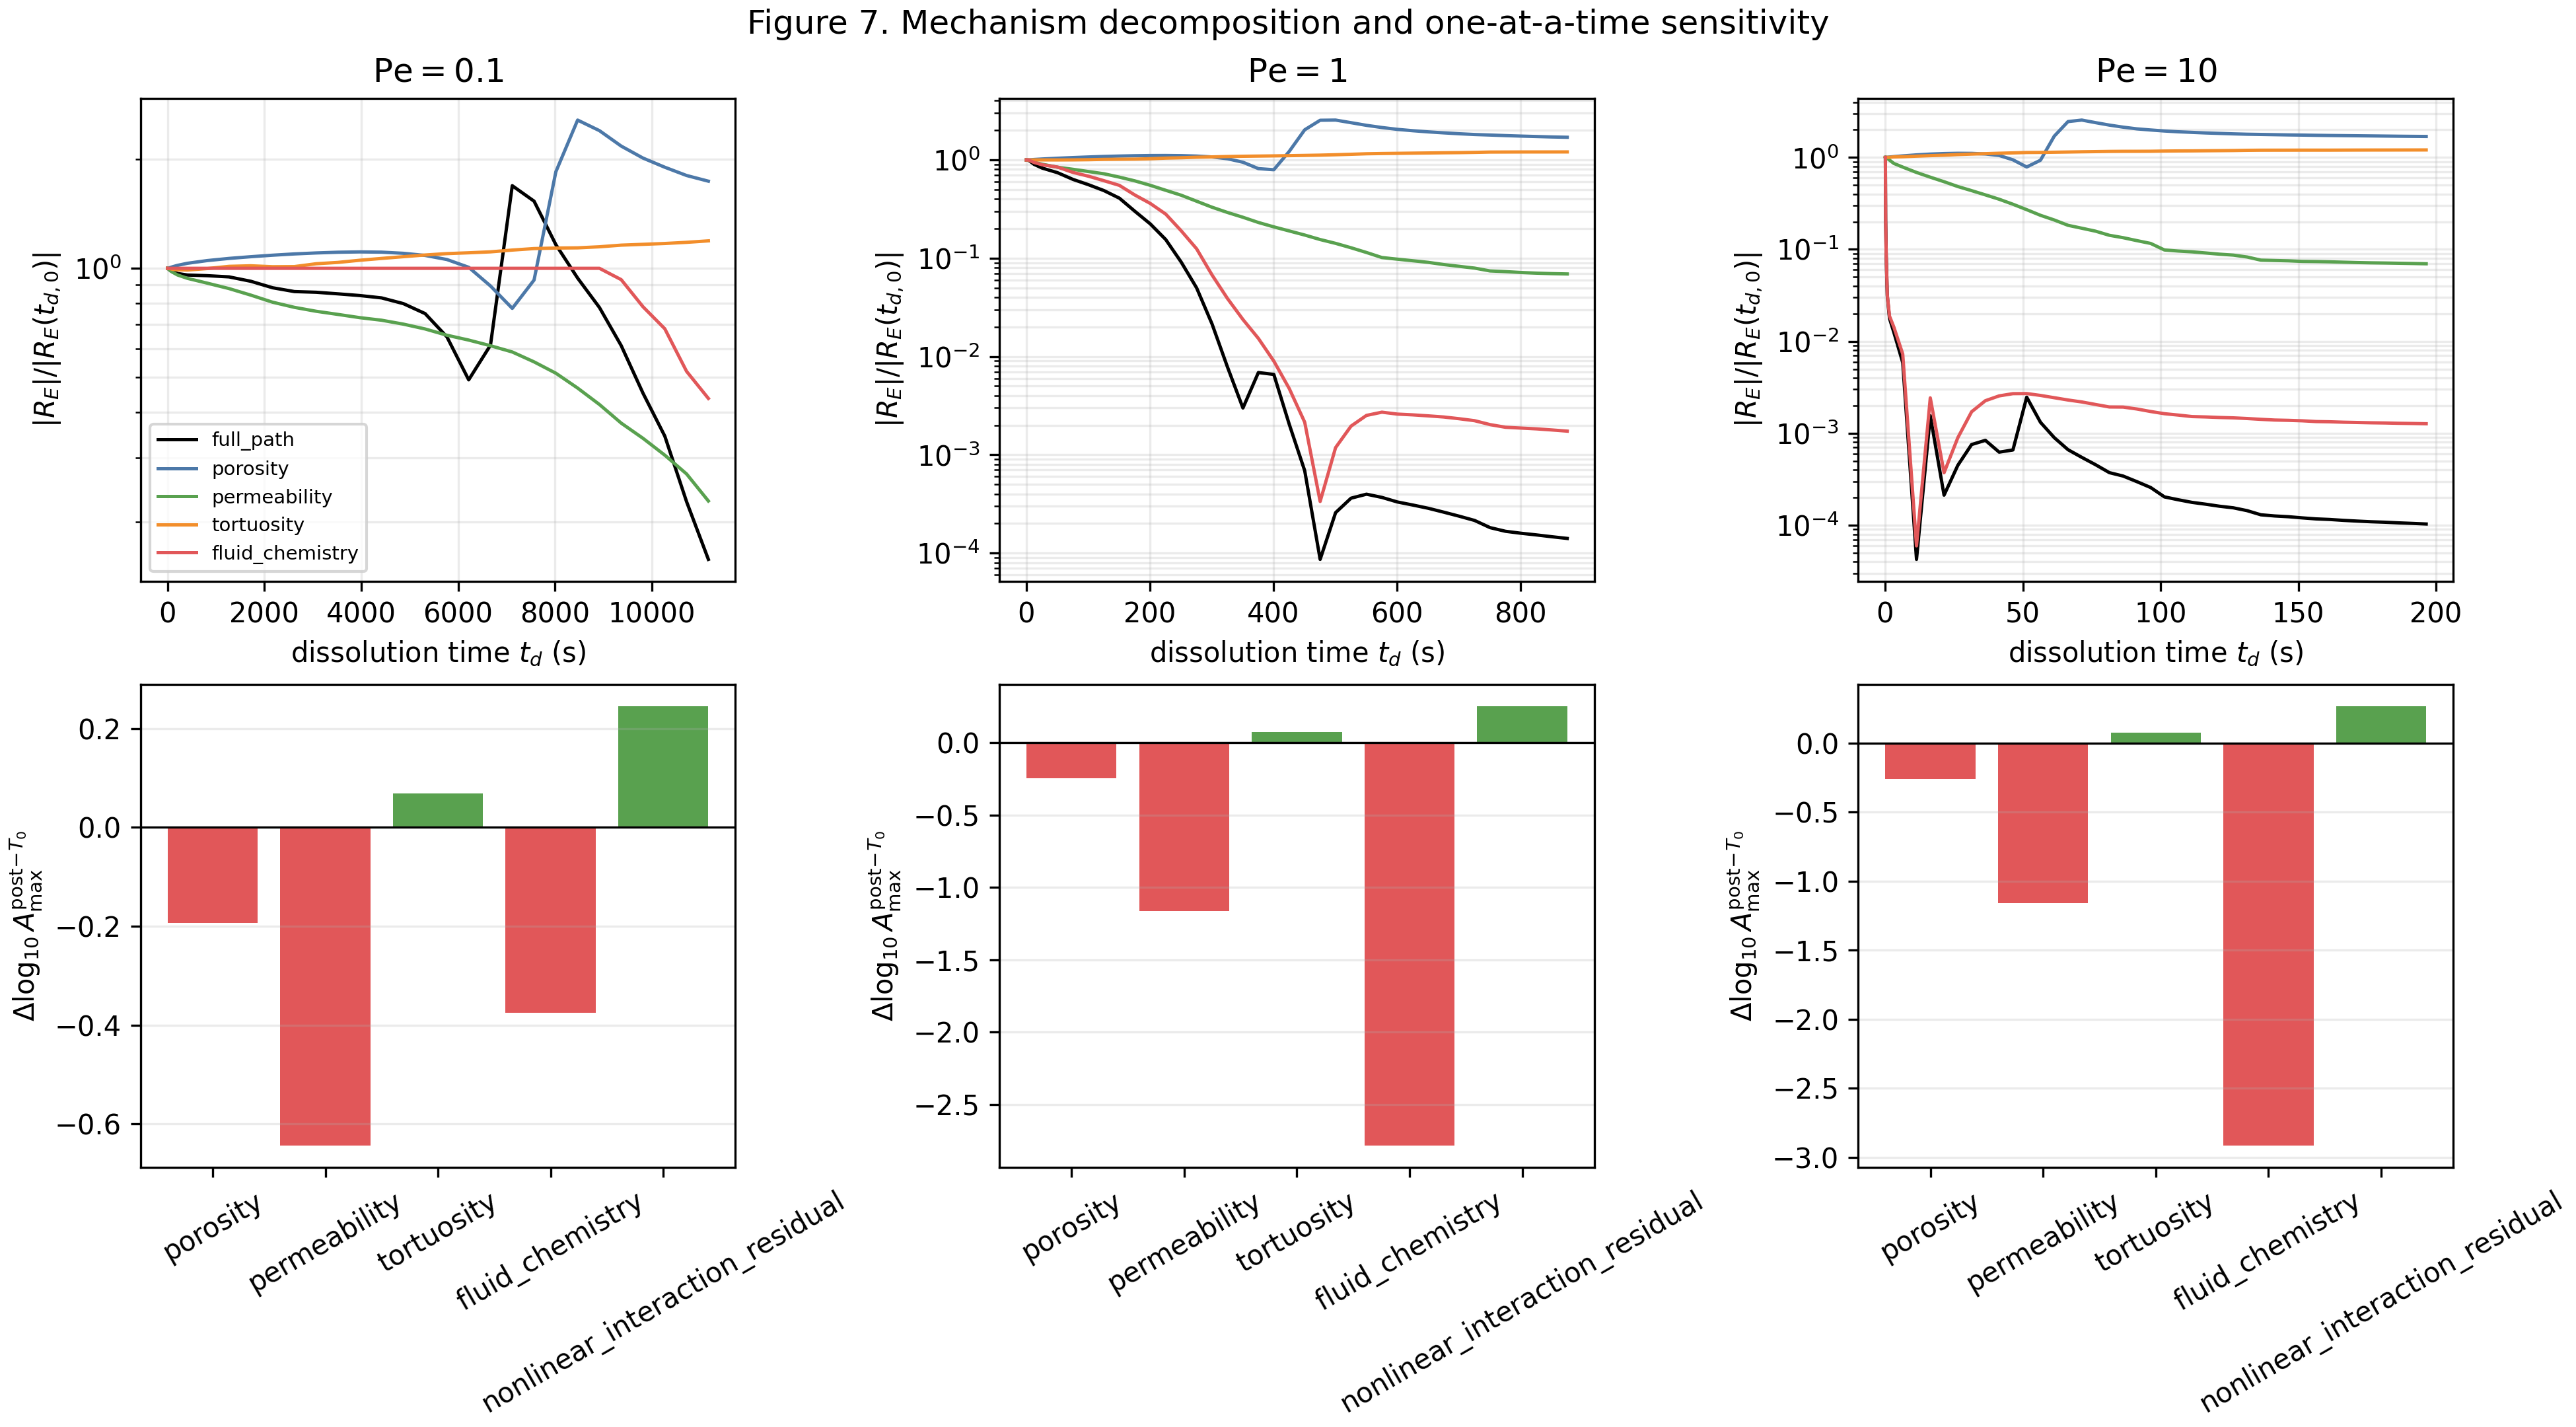
\includegraphics[width=\textwidth]{figures/figure7.png}
\caption{Mechanism decomposition using one-at-a-time parameter substitutions. The figure separates the contributions from porosity, permeability, tortuosity, and fluid chemistry pathways.}
\label{fig:mechanism_decomposition}
\end{figure}

\subsection{Normalized Metrics Provide Simulation-Based Monitoring Indicators}

Normalized $R_E$ and $|L|/|\sigma|$ decrease more strongly than the simple high-over-low frequency ratio in the higher Pe cases.
These metrics are treated as diagnostic quantities from the simulations, not as evidence of field detectability.
The normalized $R_E$ metric decreases to about 0.16 for Pe = 0.1 and to about $10^{-4}$ for Pe = 1 and Pe = 10.

\begin{figure}
\noindent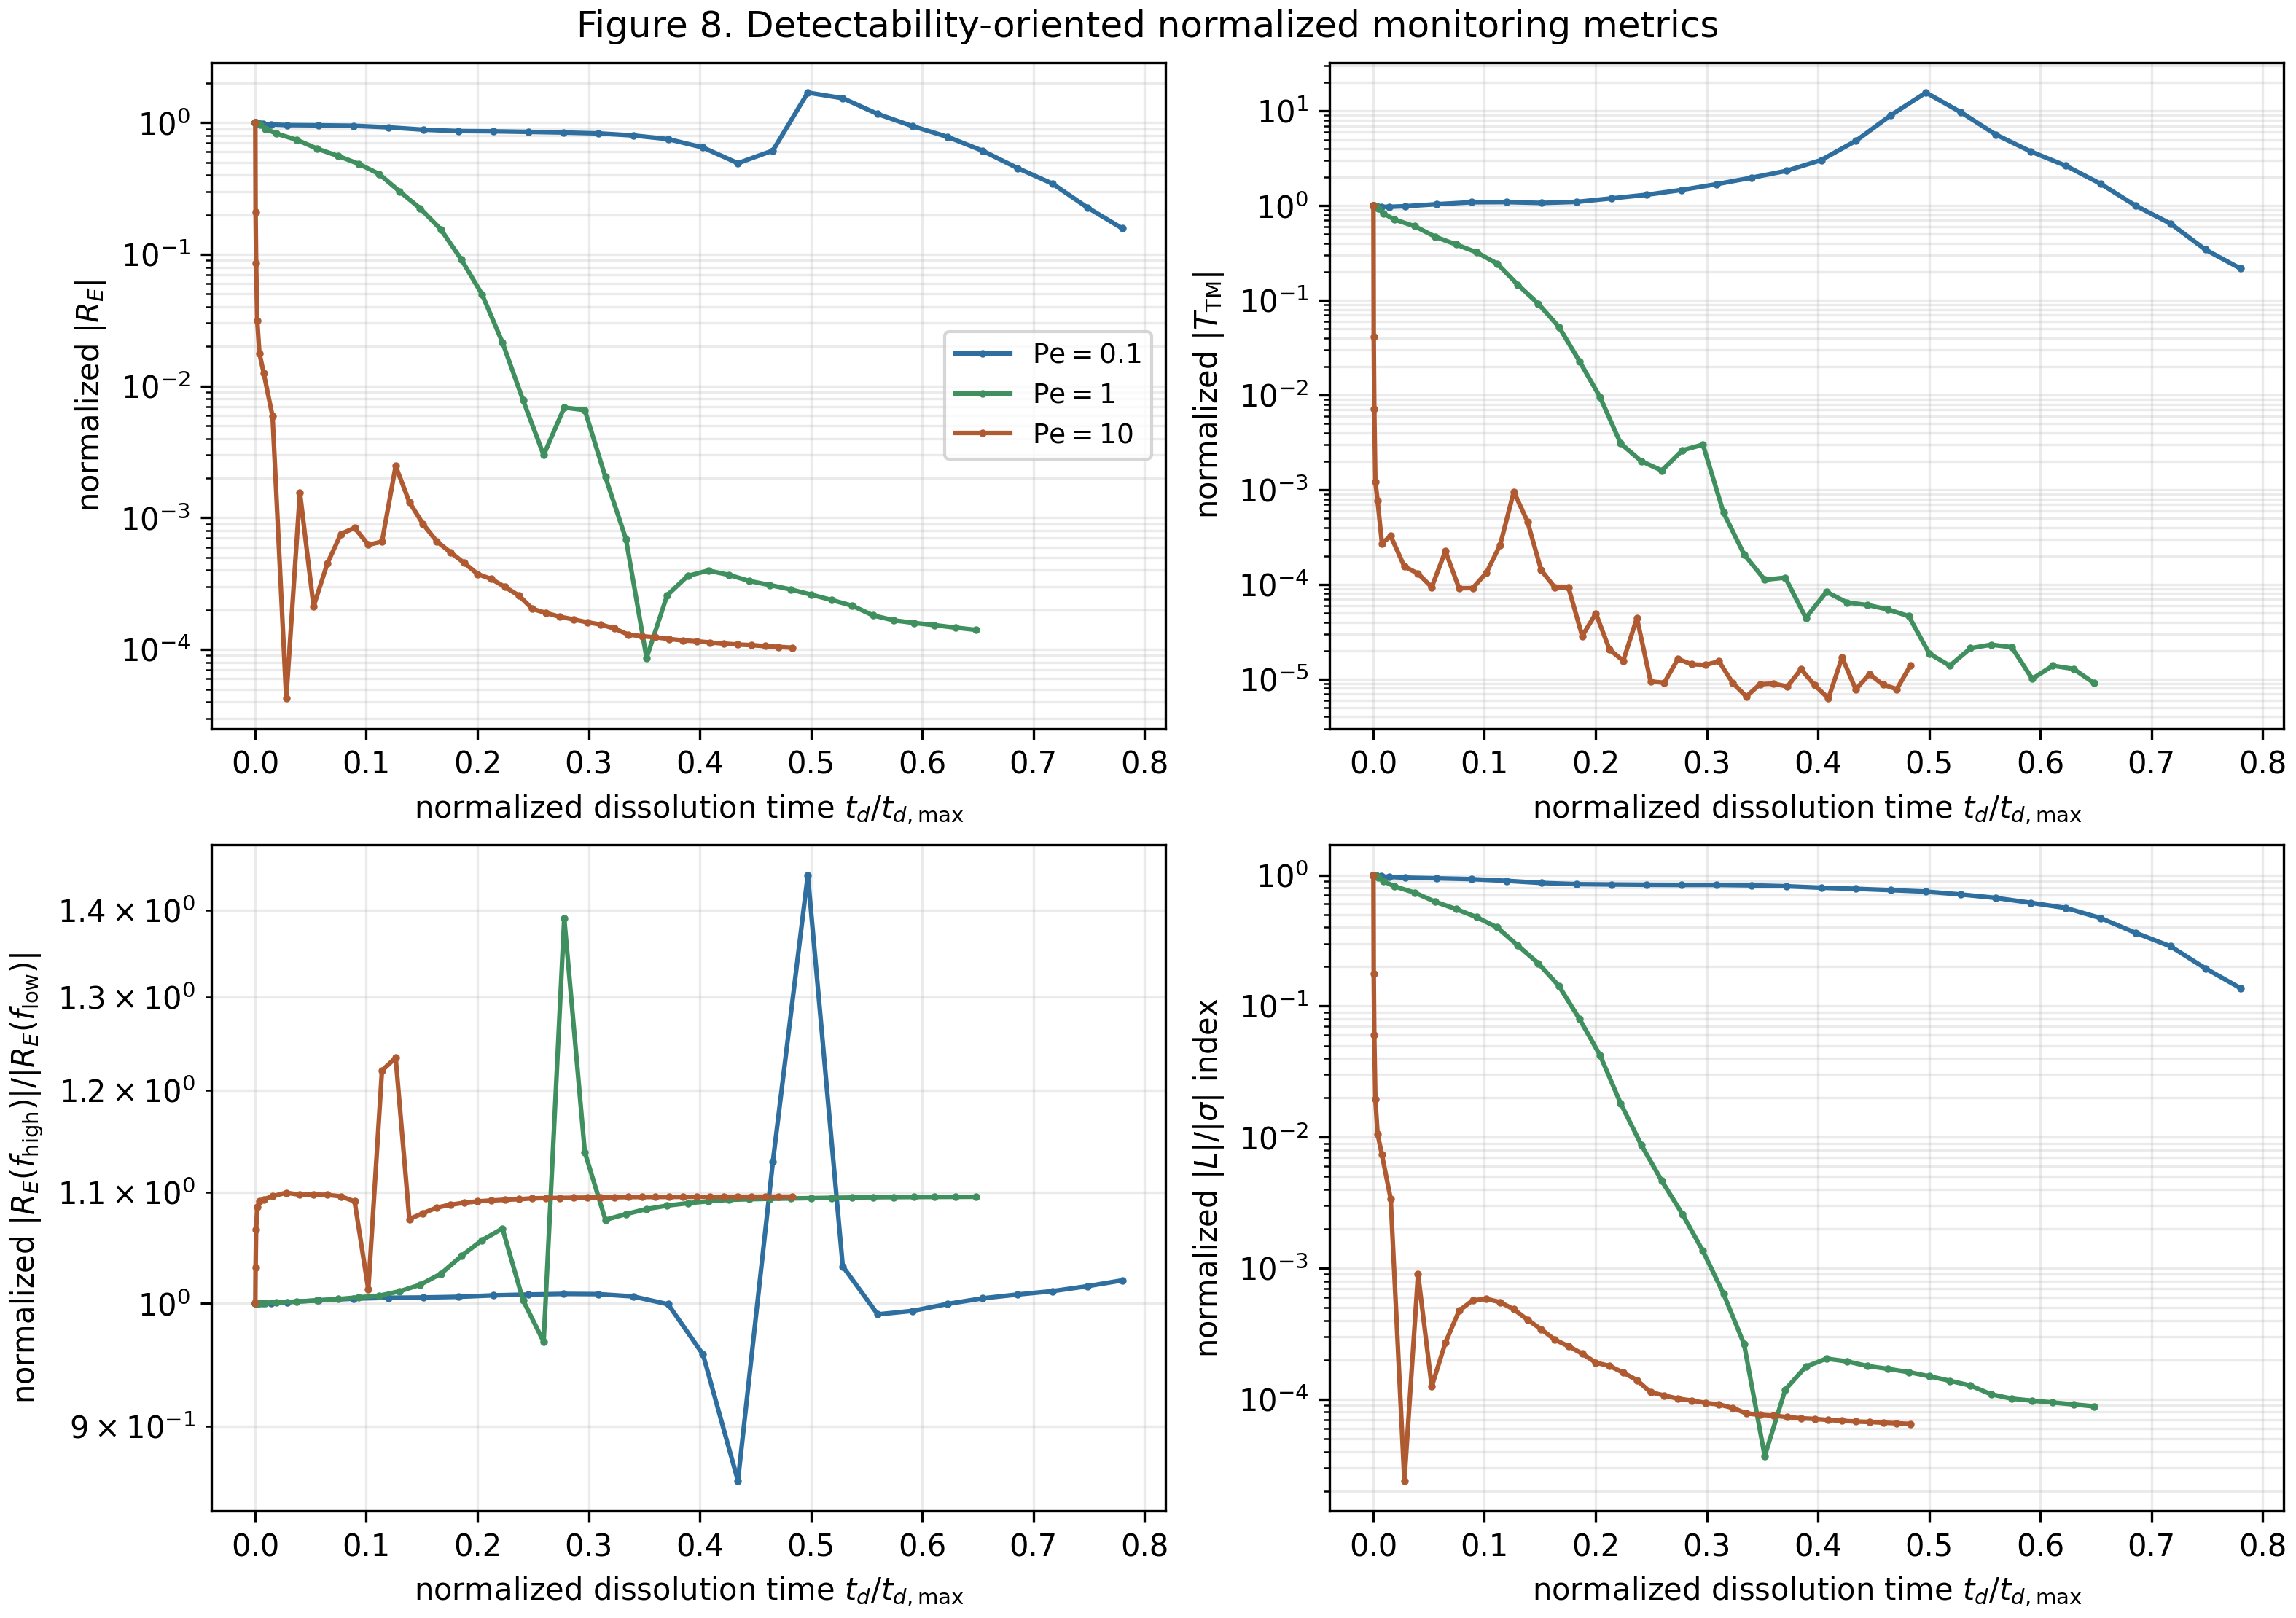
\includegraphics[width=\textwidth]{figures/figure8.png}
\caption{Normalized response metrics during dissolution. The figure compares coefficient-based and spectral-ratio indicators of response change.}
\label{fig:monitoring_metrics}
\end{figure}

\section{Discussion}

\subsection{Why Stronger Hydraulic Connectivity Can Produce a Weaker Interface Response}

The main result is not a monotonic relation between dissolution and seismoelectric amplitude.
Instead, dissolution can increase hydraulic connectivity while increasing electrical leakage, and the latter effect can dominate the interface electromagnetic source under the simulated conditions.

\subsection{Role of Peclet Number in the Coupled Response}

The Pe = 1 and Pe = 10 cases develop much larger permeability and conductivity changes than Pe = 0.1.
Their weaker interface responses indicate that transport regime affects the seismoelectric signal through coupled hydraulic and chemical pathways, not through permeability alone.

\subsection{Implications for Seismoelectric Monitoring of Reactive Systems}

The results suggest that seismoelectric monitoring of dissolution should track both hydraulic and electrical state variables.
Amplitude loss during dissolution should not be interpreted directly as reduced permeability without considering pore-fluid conductivity and coupling strength.

\subsection{Limitations and Future Work}

The present workflow uses simulated reactive transport outputs and a forward seismoelectric model, so the conclusions are limited to the tested geometry, parameter mapping, and poroelastic validity window.
Future work should separate independent fluid conductivity and $\zeta$-potential effects and compare the predicted trends with laboratory or field measurements.

\section{Conclusions}

This study links reactive transport evolution to finite-offset seismoelectric interface responses through dynamic electrokinetic properties and interface conversion coefficients.
Dissolution increases porosity and permeability, but higher Pe cases also increase pore-fluid conductivity enough to suppress $L(\omega)$, $R_E$, $T_{\mathrm{TM}}$, and post-$T_0$ waveform amplitudes.

The mechanism decomposition indicates that fluid chemistry is the main negative pathway in the strongest amplitude losses.
The practical implication is that seismoelectric response changes during dissolution should be interpreted as the outcome of competing hydraulic and electrical effects.


%%

%  Numbered lines in equations:
%  To add line numbers to lines in equations,
%  \begin{linenomath*}
%  \begin{equation}
%  \end{equation}
%  \end{linenomath*}



%% Enter Figures and Tables near as possible to where they are first mentioned:
%
% DO NOT USE \psfrag or \subfigure commands.
%
% Figure captions go below the figure.
% Acronyms used in figure captions will be spelled out in the final, published version.

% Table titles go above tables;  other caption information
%  should be placed in last line of the table, using
% \multicolumn2l{$^a$ This is a table note.}
% NOTE that there is no difference between table caption and table heading in the final, published version
%
%----------------
% EXAMPLE FIGURES
%
% \begin{figure}
% \includegraphics{example.png}
% \caption{caption}
% \end{figure}
%
% Giving latex a width will help it to scale the figure properly. A simple trick is to use \textwidth. Try this if large figures run off the side of the page.
% \begin{figure}
% \noindent\includegraphics[width=\textwidth]{anothersample.png}
%\caption{caption}
%\label{pngfiguresample}
%\end{figure}
%
%
% If you get an error about an unknown bounding box, try specifying the width and height of the figure with the natwidth and natheight options. This is common when trying to add a PDF figure without pdflatex.
% \begin{figure}
% \noindent\includegraphics[natwidth=800px,natheight=600px]{samplefigure.pdf}
%\caption{caption}
%\label{pdffiguresample}
%\end{figure}
%
%
% PDFLatex does not seem to be able to process EPS figures. You may want to try the epstopdf package.
%

%
% ---------------
% EXAMPLE TABLE
%
% \begin{table}
% \caption{Time of the Transition Between Phase 1 and Phase 2$^{a}$}
% \centering
% \begin{tabular}{l c}
% \hline
%  Run  & Time (min)  \\
% \hline
%   $l1$  & 260   \\
%   $l2$  & 300   \\
%   $l3$  & 340   \\
%   $h1$  & 270   \\
%   $h2$  & 250   \\
%   $h3$  & 380   \\
%   $r1$  & 370   \\
%   $r2$  & 390   \\
% \hline
% \multicolumn{2}{l}{$^{a}$Footnote text here.}
% \end{tabular}
% \end{table}

%%%%%%%%%%%%%%%%%%%%%%%%%%%%%%%%%%%%%%%%%%%%%%%
% SIDEWAYS FIGURES and TABLES
% AGU prefers the use of {sidewaystable} over {landscapetable} as it causes fewer problems.
%
% \begin{sidewaysfigure}
% \includegraphics[width=20pc]{figsamp}
% \caption{caption here}
% \label{newfig}
% \end{sidewaysfigure}
%
%  \begin{sidewaystable}
%  \caption{Caption here}
% \label{tab:signif_gap_clos}
%  \begin{tabular}{ccc}
% one&two&three\\
% four&five&six
%  \end{tabular}
%  \end{sidewaystable}

%% If using numbered lines, please surround equations with \begin{linenomath*}...\end{linenomath*}
%\begin{linenomath*}
%\begin{equation}
%y|{f} \sim g(m, \sigma),
%\end{equation}
%\end{linenomath*}

%%% End of body of article

%%%%%%%%%%%%%%%%%%%%%%%%%%%%%%%%%%%%%%%%%%%%%%%
%% Optional Appendices go here
%
% The \appendix command resets counters and redefines section heads
%
% After typing \appendix
%
%\section{Here Is Appendix Title}
% will show
% A: Here Is Appendix Title
%
%\appendix
%\section{Here is a sample appendix}

%%%%%%%%%%%%%%%%%%%%%%%%%%%%%%%%%%%%%%%%%%%%%%%
% Optional Glossary, Notation or Acronym section goes here:
%
% Glossary is only allowed in Reviews of Geophysics
%  \begin{glossary}
%  \term{Term}
%   Term Definition here
%  \term{Term}
%   Term Definition here
%  \term{Term}
%   Term Definition here
%  \end{glossary}


%%%%%%%%%%%%%%%%%%%%%%%%%%%%%%%%%%%%%%%%%%%%%%%
% Acronyms
%% NOTE that acronyms in the final published version will be spelled out when used in figure captions.
%   \begin{acronyms}
%   \acro{Acronym}
%   Definition here
%   \acro{EMOS}
%   Ensemble model output statistics
%   \acro{ECMWF}
%   Centre for Medium-Range Weather Forecasts
%   \end{acronyms}


%%%%%%%%%%%%%%%%%%%%%%%%%%%%%%%%%%%%%%%%%%%%%%%
% Notation
%   \begin{notation}
%   \notation{$a+b$} Notation Definition here
%   \notation{$e=mc^2$}
%   Equation in German-born physicist Albert Einstein's theory of special
%  relativity that showed that the increased relativistic mass ($m$) of a
%  body comes from the energy of motion of the body—that is, its kinetic
%  energy ($E$)—divided by the speed of light squared ($c^2$).
%   \end{notation}




%%%%%%%%%%%%%%%%%%%%%%%%%%%%%%%%%%%%%%%%%%%%%%%
%
% DATA SECTION and ACKNOWLEDGMENTS
%
%%%%%%%%%%%%%%%%%%%%%%%%%%%%%%%%%%%%%%%%%%%%%%%

\section*{Open Research Section}
The reactive transport input tables, seismoelectric modeling scripts, figure-generation scripts, and processed waveform diagnostics will be archived in a public repository before submission.
The present manuscript outline uses local files under \texttt{paper\_figure\_sequence\_analysis}; the final paper should replace this sentence with the repository DOI.

\section*{As Applicable – Inclusion in Global Research Statement}
This numerical modeling study does not currently involve field sampling, permits, or local community data.
The final manuscript should update this statement if new collaborators, field data, or institutional requirements are added.

\section*{Conflict of Interest declaration}
The authors declare that they have no conflicts of interest relevant to this manuscript.


\acknowledgments
Funding sources, computational resources, and colleagues who contributed comments or data support should be listed here.


%%%%%%%%%%%%%%%%%%%%%%%%%%%%%%%%%%%%%%%%%%%%%%%
% REFERENCES and BIBLIOGRAPHY
%
% \bibliography{<name of your .bib file>} don't specify the file extension
% don't specify bibliographystyle
%
%%%%%%%%%%%%%%%%%%%%%%%%%%%%%%%%%%%%%%%%%%%%%%%

%\bibliography{ enter your bibtex bibliography filename here }



%Reference citation instructions and examples:
%
% Please use ONLY \cite and \citeA for reference citations.
% \cite for parenthetical references
% ...as shown in recent studies (Simpson et al., 2019)
% \citeA for in-text citations
% ...Simpson et al. (2019) have shown...
%
%
%...as shown by \citeA{jskilby}.
%...as shown by \citeA{lewin76}, \citeA{carson86}, \citeA{bartoldy02}, and \citeA{rinaldi03}.
%...has been shown \cite{jskilbye}.
%...has been shown \cite{lewin76,carson86,bartoldy02,rinaldi03}.
%... \cite <i.e.>[]{lewin76,carson86,bartoldy02,rinaldi03}.
%...has been shown by \cite <e.g.,>[and others]{lewin76}.
%
% apacite uses < > for prenotes and [ ] for postnotes
% DO NOT use other cite commands (e.g., \citet, \citep, \citeyear, \nocite, \citealp, etc.).
%



\end{document}



More Information and Advice:

%%%%%%%%%%%%%%%%%%%%%%%%%%%%%%%%%%%%%%%%%%%%%%%
%
%  SECTION HEADS
%
%%%%%%%%%%%%%%%%%%%%%%%%%%%%%%%%%%%%%%%%%%%%%%%

% Capitalize the first letter of each word (except for
% prepositions, conjunctions, and articles that are
% three or fewer letters).

% AGU follows standard outline style; therefore, there cannot be a section 1 without
% a section 2, or a section 2.3.1 without a section 2.3.2.
% Please make sure your section numbers are balanced.
% ---------------
% Level 1 head
%
% Use the \section{} command to identify level 1 heads;
% type the appropriate head wording between the curly
% brackets, as shown below.
%
%An example:
%\section{Level 1 Head: Introduction}
%
% ---------------
% Level 2 head
%
% Use the \subsection{} command to identify level 2 heads.
%An example:
%\subsection{Level 2 Head}
%
% ---------------
% Level 3 head
%
% Use the \subsubsection{} command to identify level 3 heads
%An example:
%\subsubsection{Level 3 Head}
%
%---------------
% Level 4 head
%
% Use the \subsubsubsection{} command to identify level 3 heads
% An example:
%\subsubsubsection{Level 4 Head} An example.
%
%%%%%%%%%%%%%%%%%%%%%%%%%%%%%%%%%%%%%%%%%%%%%%%
%
%  IN-TEXT LISTS
%
%%%%%%%%%%%%%%%%%%%%%%%%%%%%%%%%%%%%%%%%%%%%%%%
%
% Do not use bulleted lists; enumerated lists are okay.
% \begin{enumerate}
% \item
% \item
% \item
% \end{enumerate}
%
%%%%%%%%%%%%%%%%%%%%%%%%%%%%%%%%%%%%%%%%%%%%%%%
%
%  EQUATIONS
%
%%%%%%%%%%%%%%%%%%%%%%%%%%%%%%%%%%%%%%%%%%%%%%%

% Single-line equations are centered.
% Equation arrays will appear left-aligned.

Math coded inside display math mode \[ ...\]
 will not be numbered, e.g.,:
 \[ x^2=y^2 + z^2\]

 Math coded inside \begin{equation} and \end{equation} will
 be automatically numbered, e.g.,:
 \begin{equation}
 x^2=y^2 + z^2
 \end{equation}


% To create multiline equations, use the
% \begin{eqnarray} and \end{eqnarray} environment
% as demonstrated below.
\begin{eqnarray}
  x_{1} & = & (x - x_{0}) \cos \Theta \nonumber \\
        && + (y - y_{0}) \sin \Theta  \nonumber \\
  y_{1} & = & -(x - x_{0}) \sin \Theta \nonumber \\
        && + (y - y_{0}) \cos \Theta.
\end{eqnarray}

%If you don't want an equation number, use the star form:
%\begin{eqnarray*}...\end{eqnarray*}

% Break each line at a sign of operation
% (+, -, etc.) if possible, with the sign of operation
% on the new line.

% Indent second and subsequent lines to align with
% the first character following the equal sign on the
% first line.

% Use an \hspace{} command to insert horizontal space
% into your equation if necessary. Place an appropriate
% unit of measure between the curly braces, e.g.
% \hspace{1in}; you may have to experiment to achieve
% the correct amount of space.


%%%%%%%%%%%%%%%%%%%%%%%%%%%%%%%%%%%%%%%%%%%%%%%
%
%  EQUATION NUMBERING: COUNTER
%
%%%%%%%%%%%%%%%%%%%%%%%%%%%%%%%%%%%%%%%%%%%%%%%

% You may change equation numbering by resetting
% the equation counter or by explicitly numbering
% an equation.

% To explicitly number an equation, type \eqnum{}
% (with the desired number between the brackets)
% after the \begin{equation} or \begin{eqnarray}
% command.  The \eqnum{} command will affect only
% the equation it appears with; LaTeX will number
% any equations appearing later in the manuscript
% according to the equation counter.
%

% If you have a multiline equation that needs only
% one equation number, use a \nonumber command in
% front of the double backslashes (\\) as shown in
% the multiline equation above.

% If you are using line numbers, remember to surround
% equations with \begin{linenomath*}...\end{linenomath*}

%  To add line numbers to lines in equations:
%  \begin{linenomath*}
%  \begin{equation}
%  \end{equation}
%  \end{linenomath*}
